\documentclass{report}
\usepackage[utf8]{inputenc}
%\usepackage{tikz-feynman}
\usepackage[T1]{fontenc} % Output font encoding for international characters
\usepackage{ragged2e} 
\usepackage{siunitx}
\usepackage{float}% if this breaks everything get rid 
\usepackage[style = nature]{biblatex}
\usepackage{amsmath}
\usepackage{amssymb}   % for maths symbols
\usepackage{mathrsfs}   % for maths symbols
\usepackage{todonotes}
\usepackage{graphicx}
\usepackage{caption}
\usepackage{subcaption}
\captionsetup{font=small,labelfont=bf}
\addbibresource{references.bib}
\usepackage[nottoc]{tocbibind} 
\usepackage{hyperref}


% \usepackage{geometry}
% \geometry{a4paper, total={150mm,240mm},left=30mm, top=20mm}

\usepackage[a4paper,width=150mm,top=25mm,bottom=25mm,bindingoffset=6mm]{geometry}

\graphicspath{{Dissertation/}}
\pagenumbering{arabic}




\begin{document}
%\pagenumbering{roman}
\begin{titlepage}
    \begin{center}
        \huge
        \textbf{Development of the Optical Calibration System for the Outer Detector of the LUX-ZEPLIN Dark Matter Experiment}

        
        \vspace{0.1cm}
        
    
        \LARGE
        \textbf{By\\
        \vspace{0.1cm}
        Harvey Birch\\
        \vspace{0.1cm}
         201011648}
        
        
        \vspace{1.5cm}
        
        \large
        \textbf{Supervisors: Dr Sergey Burdin and Dr Will Turner}
        
        
        \normalsize
        A report submitted in partial fulfillment of the requirements for the degree of\\
        \vspace{0.5cm}
        \large
        \textbf{Particle Physics MPhil}
        
        \vspace{0.3cm}
        
    
        \large
        Department of Physics\\
        \vspace{0.3cm}
        University of Liverpool\\
       
        
       
        June 2019
        
        \vspace{1cm}
        \begin{figure}[h]
            \centering
            
\includegraphics[width=0.7\textwidth]{Figures/UoL.png}
        \end{figure}
        \begin{figure}[h]
            \centering
            \includegraphics[width=0.25\textwidth]{Figures/LZ_logo.png}
        \end{figure}
        
        
    \end{center}
\end{titlepage}
\pagenumbering{roman}
\tableofcontents
\listoffigures
\listoftables
\pagenumbering{arabic}
\chapter{Introduction}\label{Chap1:Intro}
\setcounter{page}{1}
Over the last $\sim150$ years physicists have observed discrepancies between astronomical measurements and the observations of luminous matter (\S\ref{Chap2:Cosmo}). Many postulate that the existence of Dark Matter in our Universe is the reason for these discrepancies. Application of the virial theorem along with measurements of galaxy velocity have been used to determine the mass of galaxies, such calculations differ to expected mass given the observed luminosities. Similar differences can be seen when using gravitational lensing, where the mass of an astronomical objects be reconstructed and the expected mass determined by the object's luminosity differ. The ratio of mass-light can be used to estimate the amount of Dark Matter in cosmological structures throughout our Universe. The distribution of energy throughout our universe can be also estimated using cosmological models such as the $\Lambda$CDM model. Using the most recent observations \cite{Planck2018} and measurements \cite{WMAP}, the energy distribution of Universe can be estimated to be: $\sim5\%$ Baryonic matter;$\sim26\%$ Dark Matter; and $\sim69\%$ Dark Energy. With Dark Matter constituting over a quarter of the energy/mass in our Universe, these estimates provide the motivation to investigate and understand it's properties. 
\newline
Of the possible candidates for Dark Matter (\S\ref{Chap3:Candi}), Weakly Interacting Massive Particles (WIMP's) are currently seen to be one of the more viable candidates by the scientific community. The LUX-ZEPLIN (LZ) experiment will probe the parameter space of the WIMP via direct detection (\S\ref{sec:directdetection}) using a liquid noble gas approach. The experiment aims to push the limits of the WIMP cross section close to the neutrino floor. Building on the success of it's predecessor, LUX \cite{LUX}, LZ will utilise a liquid Xenon time projection chamber (LXe-TPC) (\S\ref{sec:TPC}) and hopes to achieve greater sensitivity with the addition of Outer Detector (OD). The OD will be instrumented as a veto system to rejected unwanted signals within the LXe-TPC. (\S\ref{sec:veto}). The High Energy Particle group at the University of Liverpool are responsible for the development and production of the Outer Detector Optical Calibration System (OCS).
\newline
This report will present a short literature review to outline the motivations to search for Dark Matter, the possible candidates and the methods in which the candidates could be found. Then the detection method LZ will utilise and it's veto system will be described (\S\ref{Chap5:LZ}). The Outer Detector Optical Calibration System will be described (\S\ref{Chap6:OCS}), followed by an explanation of the tests which were performed on the system throughout it's development (\S\ref{Chap7:FST}). The Fibre Support Structures (FFS) used within the OD to align the injection points will be demonstrated (\S\ref{Chap8:FSS}). An investigation will take place into the development of an insert that will be used in the FFSs to hold the fibre in place (\S\ref{sec:FSSID}). A discussion about the future development of the OCS will also be made (\S\ref{Chap10:Discussion}). 

\chapter{Cosmological indications for Dark Matter}\label{Chap2:Cosmo}
Historically, the term "Dark Matter" was incorrectly used to explain discrepancies in measurements of the movement of stars within the Milky Way Galaxy by Jacobus Kapteyn. In 1933 Fritz Zwicky observed unexpectedly high velocities of nebulae in the Coma cluster. He applied the virial theorem to the observations to find that there was 400 times more mass calculated than was visibly observed. The effect of gravity in the cluster was also far too small for visible matter which was moving at such high velocities. After taking into account the discrepancy in mass and gravity, Zwicky inferred the existence of Dark Matter which would "hold" the cluster together \cite{Zwicky1933}. 
\newline
Another indication for existence of Dark Matter is the observed effect of gravitational lensing \cite{GravLens}. It was first described by Albert Einstein in 1936 \cite{Einstin1936} and was further studied by Zwicky in 1937 \cite{Zwicky1937}. The effect occurs when a massive object is situated in the line of sight between the observer and the object being observed. Due to the gravitational field of the massive object, light rays deflect from their path resulting in a deformation or in multiple images of the object being studied. The gravitational potential of the massive object can be reconstructed using the degree of deformation of the light. The mass of the object in the line of sight can also be reconstructed using this method and from observations it is found that the reconstructed mass is 200 times greater than the luminous matter observed.
\newline
Further discrepancies in the mass to light ratio measured by Horace W. Babcock in 1939 in his study of galaxy rotation curves \cite{RotationCurves}. His study of the Andromeda Galaxy suggested that the mass to light ratio increased radially due to light absorption within the galaxy. It was not until Jan Oort discovered a non-visible halo, NGC 3115, in 1940 which could be used to explain rotation curves within Andromeda \cite{Oort1940}. In 1978 Vera C. Rubin \textit{et al.}\cite{Rubin} studied a sample of 10 high-luminosity spiral galaxies, to find that the rotation velocities of stars in the galaxies would remain constant as the distance from the galactic centre increased. This was a contradiction to the expected result from Newtonian Dynamics which states that objects outside the visible mass distribution should have velocities $v \propto 1/\sqrt{r}$. The presence of a Dark Matter halo distributed uniformly throughout a galaxy could explain the observed phenomena.
\newline
The presence of Dark Matter in our universe can be shown using the $\Lambda$CDM model which consists of six parameters \cite{LCDMparam}. The model takes into account high sensitivity small angular resolution measurements in the infra-red spectrum from the Planck space observatory \cite{Planck2018} and fluctuations in Cosmic Microwave Background (CMB) radiation early on in our universe, observed by the Wilkinson Microwave Anisotropy Probe (WMAP) \cite{WMAP}. The model is fitted to the cosmological observations and measurements to determine some of the model's parameters.
The model's six parameters are physical baryon density parameter, physical Dark Matter density parameter, the age of the universe, scalar spectral index,  the amplitude of the initial fluctuations and re-ionisation optical depth \cite{LCDMparam}.The most recent estimates from Planck 2018 \cite{Planck2018} allow a calculation of the mass-energy distribution in our universe. The analysis shows a spatially-flat flat universe with $\Omega_B = 0.049$, $\Omega_{DM} = 0.265$ and $\Omega_\Lambda = 0.686$ representing the densities of baryonic matter, Dark Matter and Dark Energy. 
\newline
It is postulated that the anisotropies of the CMB arose from quantum fluctuations in matter during inflation of the early universe. The concentration of Dark Matter density increased as the fluctuations propagated through the universe during the inflation, as the baryonic matter in the concentration cooled cosmological structures formed due to increasing gravitational forces. The evolution of the Universe has been simulated and has accurately reproduced the measurements produced by galaxy surveys such as those of the Lyman-$\alpha$ Forest. Simulations have also reproduced the effects of weak lensing to confirm the cosmic structure taking into consideration non-luminous and non-baryonic matter as well as galaxies and gas clouds \cite{GravLens}. 

\chapter{Possible candidates for Dark Matter}\label{Chap3:Candi}
One probable solution to explain the discrepancies in the mass to light ratio discussed in chapter \ref{Chap2:Cosmo} is to assume there is no Dark Matter present, and a modification of Newton's gravitational laws is needed to yield the observed results. Modifications such as MOND \cite{MOND} and TeVeS \cite{TeVeS} attempt to solve the problem in a classical and relativistic manner respectively, both failing to do so independently. MOND fails to explain the observations on the structure of CMB whilst also violating some of the fundamental laws. Whereas TeVeS successfully solves the problems encountered by MOND but fails to describe rotation curves and gravitational lensing.
Another possible explanation for large mass to light ratios could be the presence of Massive Astrophysical Compact Halo Objects (MACHOs) which emit little to no radiation. MACHOs could come in the form of neutron stars, black holes, brown dwarfs or un-associated planets. No suitable MACHO candidates have been found using gravitational microlensing \cite{MicroLens}. Baryonic nature of Dark Matter can also be ruled out due the Big-Bang nucleosynthesis (BBN)\cite{BBN}.
\newline
One of the more widely accepted and well motivated candidates for Dark Matter is in the form of a Weakly Interacting Massive Particle (WIMP). An assumption is made such that in the early universe WIMP's were in equilibrium with the cosmic plasma. During the expansion of the universe, the plasma cooled to a temperature lower than that of the WIMP mass leading to the decoupling from the plasma \cite{DMProd}. The Dark Matter relic density was reached at this freeze-out temperature when the WIMP annihilation rate became less than the Hubble expansion rate. The cross-section needed to detect a particle in the current Dark Matter density is of the order of the weak interaction scale, giving theoretical reason for motivation to search for a WIMP-like particle. 
\newline
The only suitable candidate from Standard Model to be considered would be the neutrino. It would be be thought as a "hot" Dark Matter candidate due to it's relativistic velocity in the early universe. But due to neutrino's fermionic nature and constraints set by the Fermi-Boltzmann distribution, they cannot account for the Dark Matter density within halos \cite{DirectDetection2015}. The hypothetical, Sterile Neutrino, introduced to explain the size of a neutrino mass could provide a possible candidate for Dark Matter. They could either be a cold (always non-relativistic) or a warm (only relativistic in the early universe) Dark Matter candidate depending on their production mechanism. Unfortunately due to the low mass and interaction strength a sterile neutrino would be difficult to detect directly. 
\newline
As well as WIMP's and neutrinos, axions are another form of particle which could be a candidate to solve the Dark Matter problem. The axion particle was postulated in 1977 \cite{ConsvCP} to solve the "strong CP-problem" due to P and CP violation from the experimental bound on the neutron dipole moment \cite{NeutronDi}. Axion-like particles would have been produced in the early Universe in mechanisms such as vacuum realignment \cite{InvisAx}. Due to a small free streaming length, the axion is considered a "cold" Dark Matter candidate. 
\newline
The candidates discussed in this chapter were not originally proposed to solve the Dark Matter problem, but with the motivation to provide solutions to other models and theories in physics. This external motivation only strengthens the importance of the candidates. A more detailed discussion of of the evidence and candidates for Dark Matter can be found in \cite{DMCandidates}.

\chapter{Searches for Dark Matter}\label{Chap4:Search}
Searching for particle Dark Matter can be done using three mechanisms: indirect detection by searching for signals from annihilation products; production at particle colliders and direct detection via scattering off target nuclei. Figure \ref{fig:detection_schem} illustrates the possible Dark Matter detection methods and how an ordinary matter particle, P, would couple to a potential Dark Matter candidate, $\chi$.
\begin{figure}[h]
    \centering
    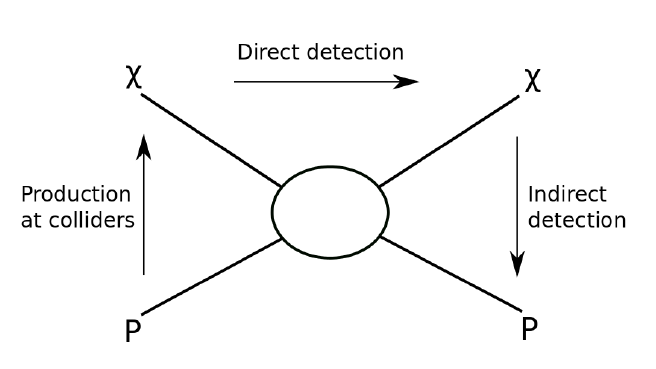
\includegraphics[width=0.7\textwidth]{Figures/Detection_schematic.png}
    \caption{Schematic illustrating the three possible Dark Matter detection methods: production of Dark Matter particles from the collision of ordinary matter (upwards); detection of recoil products (left to right); and dark matter particles annihilating to produce ordinary matter (downwards) \cite{DirectDetection2015}}
    \label{fig:detection_schem}
\end{figure}
\section{Indirect detection of Dark Matter}\label{sec:indirect}
An increase in Dark Matter density form halos around astronomical objects such as stars and galaxies which make these sources ideal regions in which to conduct indirect Dark Matter searches. The Dark Matter flux produced in these regions of higher density could be used to measure its presence due to scattering, self annihilation and decays into standard model particles. By detecting these decay products, it could infer the existence of Dark Matter. The possible decay channels can be seen in equations \ref{eqn:DMGAMMA} and \ref{eqn:DMBARY} \cite{DMProd}:
\begin{equation}\label{eqn:DMGAMMA}
    \chi\Bar{\chi} \rightarrow \gamma\gamma,\: \gamma Z,\: \gamma H \quad \textrm{or}
\end{equation}
\begin{equation}\label{eqn:DMBARY}
    \chi\Bar{\chi} \leftrightarrow e^+e^-,\: \mu^+\mu^-,\: q\Bar{q},\: W^+W^-,\: ZZ,\: HH\: ...
\end{equation}
There are many other possible indirect detection mechanisms that can be searched for such as observing high energy $\gamma-\textrm{rays}$ using atmospheric Cherenkov telescopes pointed in the direction of objects with expected high levels of Dark Matter or detecting neutrinos which radiate out of the sun after capture \cite{DirectDetection2015}. 

\section{Dark Matter production at colliders}\label{sec:colliders}
The production of Dark Matter at particle colliders is a well motivated method in which observing events with missing transverse momentum and energy would infer the possible presence of a WIMP. Since 2008, the ATLAS and CMS experiments on the Large Hadron Collider at CERN have used proton-proton collisions with a centre of mass energy of $7\:TeV\textrm{ to }13\:TeV$ to search for new particles. The mechanism in which a particle collider would detect a WIMP-like can be seen in equation \ref{eqn:DMCOLLIDER} where $p$ represents proton and $x$ could be either a hadronic jet, a photon or leptonically decaying Z or W boson \cite{DirectDetection2015}.
\begin{equation}\label{eqn:DMCOLLIDER}
   pp \rightarrow \chi\Bar{\chi} + x
\end{equation}
Results remain consistent with standard model expectations from analysis of the data from collision events. With the forthcoming upgrade of the LHC, increased luminosity's and collision energies will allow for a larger parameter space to be analysed.

\section{Direct detection of Dark Matter}\label{sec:directdetection}
The direct detection of Dark Matter involves the identification of nuclear recoils produced from the collision of Dark Matter particle, a WIMP, with a detector's target nuclei. The nuclear recoils observed would be in the range of $1-100\:keV$ from a collision of WIMP with a mass of $10-1000\:GeV/c^2$ \cite{DirectDetection2015}. The signal produced by the nuclear recoil can be observed by one of three different forms: phonons or heat; charge; and light. A detector will be designed with the corresponding technologies to detect one or two of the possible three signals. A schematic of this process can be seen in figure \ref{fig:Direct}.
\begin{figure}[h]
    \centering
    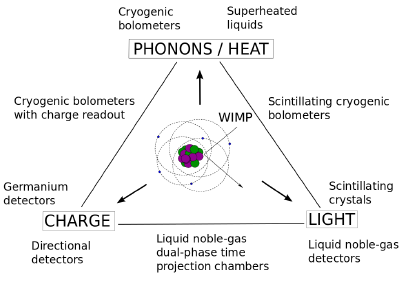
\includegraphics[width=0.7\textwidth]{Figures/Direct_direction.png}
    \caption{A schematic showing the possible direct detection signals and the corresponding experiments used to observe such signals.\cite{DirectDetection2015}}
    \label{fig:Direct}
\end{figure}
The LUX-ZEPLIN (LZ) experiment will observe signals of both light and charge by utilising a liquid Xenon dual phase time projection chamber, this method will be described in chapter \ref{Chap5:LZ}.
\newline
The three different detection techniques discussed in this chapter collectively cover the range set on the parameter space in which the WIMP cross-section lies. If one of the methods were to be successful in identifying a WIMP, the result would then be verified with one or combination of the two remaining methods.

\chapter{LUX-ZEPLIN Experiment}\label{Chap5:LZ}
LZ is a second generation Dark Matter direct detection experiment. The detector will operate in Sanford Underground Research Facility in South Dakota, USA \cite{SURF}. At the core of the LZ experiment there is a two-phase Time Projection Chamber (TPC) containing seven fully active tonnes of liquid Xenon (LXe). The TPC is enclosed by a Xenon Skin, acrylic tanks filled with liquid scintillator and an water tank housing 120 PMTs. The detector will be located in the existing 250-ton water tank used by LUX. LZ will use a total liquid xenon mass of 10 tonnes, an active mass of 7 tonnes and a fiducial mass of 5.6 tonnes \cite{LZTDR}. Over a 3 year period of operation, the experiment will probe WIMP-nucleon cross sections down to $2 \times 10^{-48} cm^2$ at 100 GeV \cite{LZIntro}. A drawing of the LZ detector can be seen in Figure \ref{fig:LZDetector}. 
\begin{figure}[h]
\centering
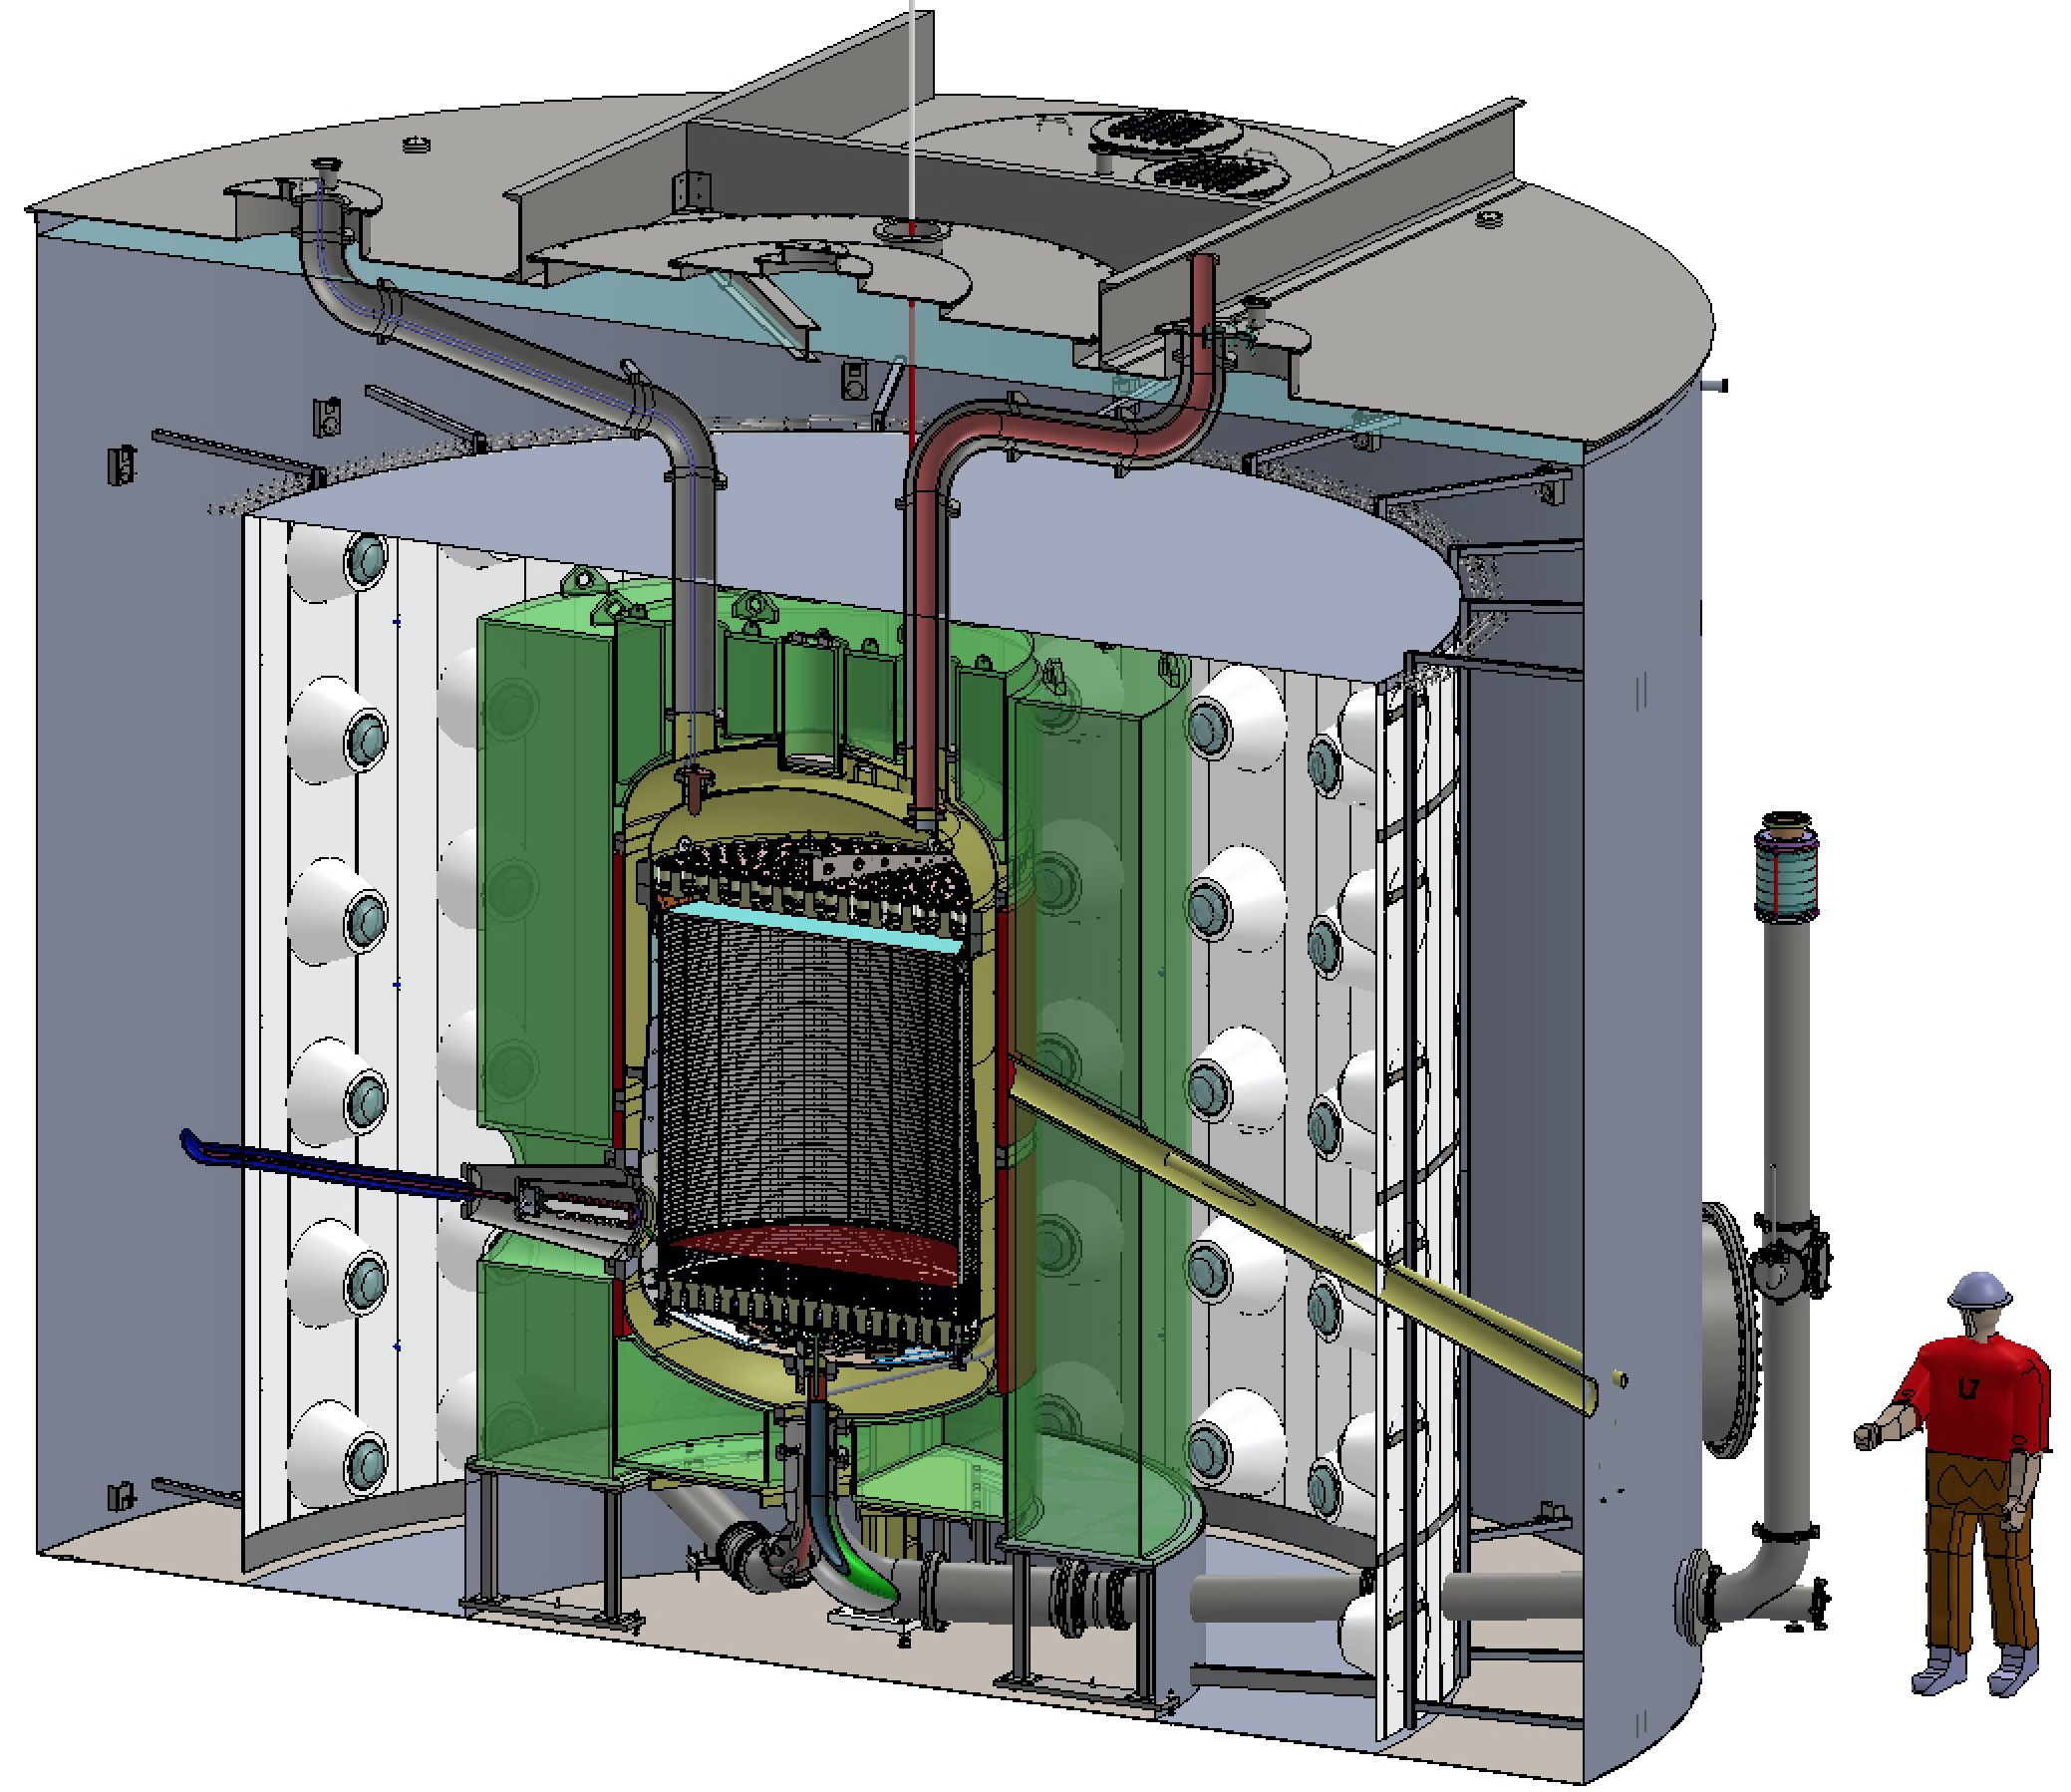
\includegraphics[width=0.7\textwidth]{Figures/Detector_design.jpg}
\caption{Cutaway drawing of the LZ detector systems. The LXe TPC is surrounded by the xenon skin layer (yellow), the scintillator tanks (green) and light collection system (white), all housed in a large water tank (blue-grey).\cite{LZTDR}}
\label{fig:LZDetector}
\end{figure}

\section{Dual phase LXe TPC}\label{sec:TPC}
As mention previously, the experiment will use a LXe TPC to detect a WIMP. After a WIMP interacts with a LXe atom in the TPC two signals are generated. In this interaction prompt scintillation light (S1) is produced from a nuclear recoil, this recoil also causes the ionisation of neighbouring atoms which produces free elections. These free elections are drifted upwards through the TPC using an induced electric field to the surface of the LXe, the free electrons are extracted in a gaseous phase and accelerated to produce a second scintillation signal (S2). Two arrays of photomultiplier tubes (PMTs), 253 on the top and 241 on bottom of the TPC measure the signals \cite{LZTDR}. The difference in time between the S1 signal and S2 signal is used to calculate the z-position in which the interaction occurs, the x-y position is determined by distribution of the S2 signal in the upper array of PMTs. The ratio of S2/S1 signals can be used to discriminate between different background sources and WIMP particles. A schematic of detection mechanism in dual phase TPC can be seen in figure \ref{fig:TPC_mech}. 

\begin{figure}[h]
    \centering
    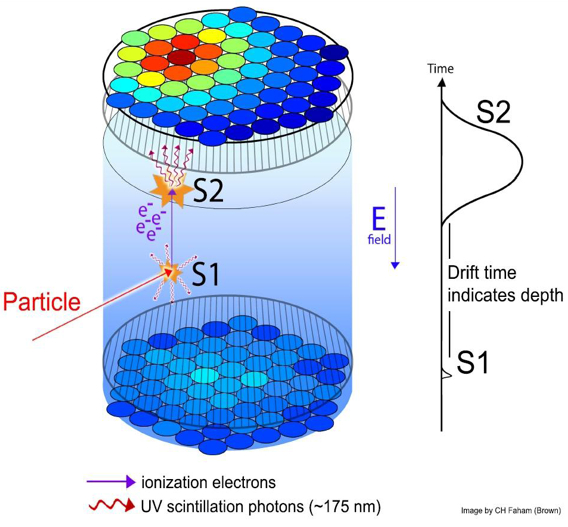
\includegraphics[width=0.6\textwidth]{Figures/TPC_mechanism.jpg}
    \caption{A schematic illustrating the principle in which a dual phase LXe TPC detects a WIMP interaction. When particle (WIMP) interacts with a LXe atom two signals are produced. The first signal produced is prompt scintillation light (S1) and the second signal produced are free electrons from the ionisation of neighbouring LXe atoms. The difference in time between S1 and S2 signal can be used to determine the z-position of the interaction and the distribution of light in the upper PMT array from the S2 signal can be used to determine the x-y position.  \cite{DMUCL}}
    \label{fig:TPC_mech}
\end{figure}

\section{Veto system}\label{sec:veto}
The TPC containing the large active volume of LXe is surrounded by a three-component veto system used to reject and characterise the background radiation from the surrounding environment. The first component of the veto system is the Xenon skin region located between the TPC and the cryostat walls, containing three tonnes of LXe, monitored by 131 PMTs. The second component of the veto system is ten acrylic tanks filled with seventeen tonnes of Gadolinium-loaded Liquid Scintillator (Gd-LS)\cite{LZTDR}.
The primary role of the scintillator is to tag neutrons which could cause nuclear recoils with a similar signature to that produced by WIMPs within the TPC. When the neutrons interact with the Gd-LS, scintillation light is produced and detected by an array of 120 8 inch Hamamatsu R5912 PMTs which surround the acrylic tanks. The third component of the veto system is ultra pure water surrounding the acrylic tanks. The ultra-pure water is used as a muon veto and shielding. The OD of LZ consists of the Gd-LS tanks, volume of water and is monitored by 120 PMT's
\newline
The layout of veto system can be seen in figure \ref{fig:LZDetector} where the Xenon skin layer is highlighted yellow, the Gd-LS Scintillator tanks in green and the PMT array mounted on a reflective screen of Tyvek\textregistered. An in depth description of the detector can be found in the LUX-ZEPLIN Technical Design Report (TDR) \cite{LZTDR}. In 2014, the University of Liverpool High Energy Particle group joined the LUX-ZEPLIN experiment. The group are responsible for the Optical Calibration System that will be used to calibrate the PMTs in the Outer Detector. This system will be discussed in chapter \ref{Chap6:OCS}. 

\chapter{Optical Calibration System}\label{Chap6:OCS}
LZ will use an Optical Calibration System (OCS) to monitor the performance of the OD. Light will be injected into the OD using an LED-driven system with 30 duplex optical fibres mounted within the array of PMTs and 5 duplex optical fibres mounted beneath the tanks. The injection points situated within the array will maintain calibration of PMTs and monitor their performance. The light transmission of the acrylic tanks will be monitored by the 5 bottom injection points. A schematic illustrating the locations of some of the inject points can be seen in figure \ref{fig:inject}. The OCS will have the capability to inject light from a threshold of $\approx 100 keV_{ee}$ up to $\sim 10 MeV_{ee}$, this range will account the signals produced by neutron capture within the scintillator as well as the large signals from penetrating cosmic muons \cite{LZTDR}. Gain drift of the OD PMTs will be monitored injecting a set number of photons during each calibration and measuring the light collection at each PMT. The gain of the PMTs will be adjusted to ensure consistent light collection throughout the running of the experiment.

\begin{figure}[h!]
    \centering
    \includegraphics[width=0.7\textwidth]{Figures/OD_CUT_THROUGH.png}
    \caption{A schematic of a cut through of the OD were some of the injection points are highlighted in red. Each injection point located at the centre of 4 PMTs.}
    \label{fig:inject}
\end{figure}

\section{System requirements}\label{list:SystemReq}
The requirements for the OCS outlined in the main LZ requirements document are;
\begin{itemize}
    \item Number of photons per CH, 700-50 k photons.
    \item Number of photons globally, 1 M photons.
    \item Pulse variation at level of statistical variation in the OD.
    \item Variation calibration to calibration $< \sim100$ photons at 150 keV.
    \item Calibration steps: 700 - 1200 photons: 100 photons step; 5 - 10k: 1k step.
    \item Pulse width, $< 20$ ns.
    \item Pulsing frequency up to 10 kHz.
    \item Light pulse wavelength: 430-450 nm, 450-460 nm, 365-390 nm.
    \item Alignment, $<5\deg$ misalignment.
\end{itemize}

\section{System overview}
The OCS electronics system consists of 5 Optical Calibration Cards (OCC). Each card consists of a FPGA motherboard, which houses 8 LED pulser boards as well as 2 photo-diode read-back boards. Light from the LED's is fed to the front panel and a photo-diode via a 3-way optical coupler. The components of a OCC can be seen in figure \ref{fig:OCC}. The electronics system for the OCS will interface will the detector via 40 duplex optical fibres which will enter the water tank via an air tight and light tight feed-through port on the top of the tank. The light produced by the system will be monitored by two methods, firstly by two four-channel photo-diode daughter boards controlled by the FPGA board and secondly by a rack mounted calibration PMT (identical to the Hamamatsu R5912 PMTs used in the Outer Detector).

\begin{figure}[h]
    \centering
    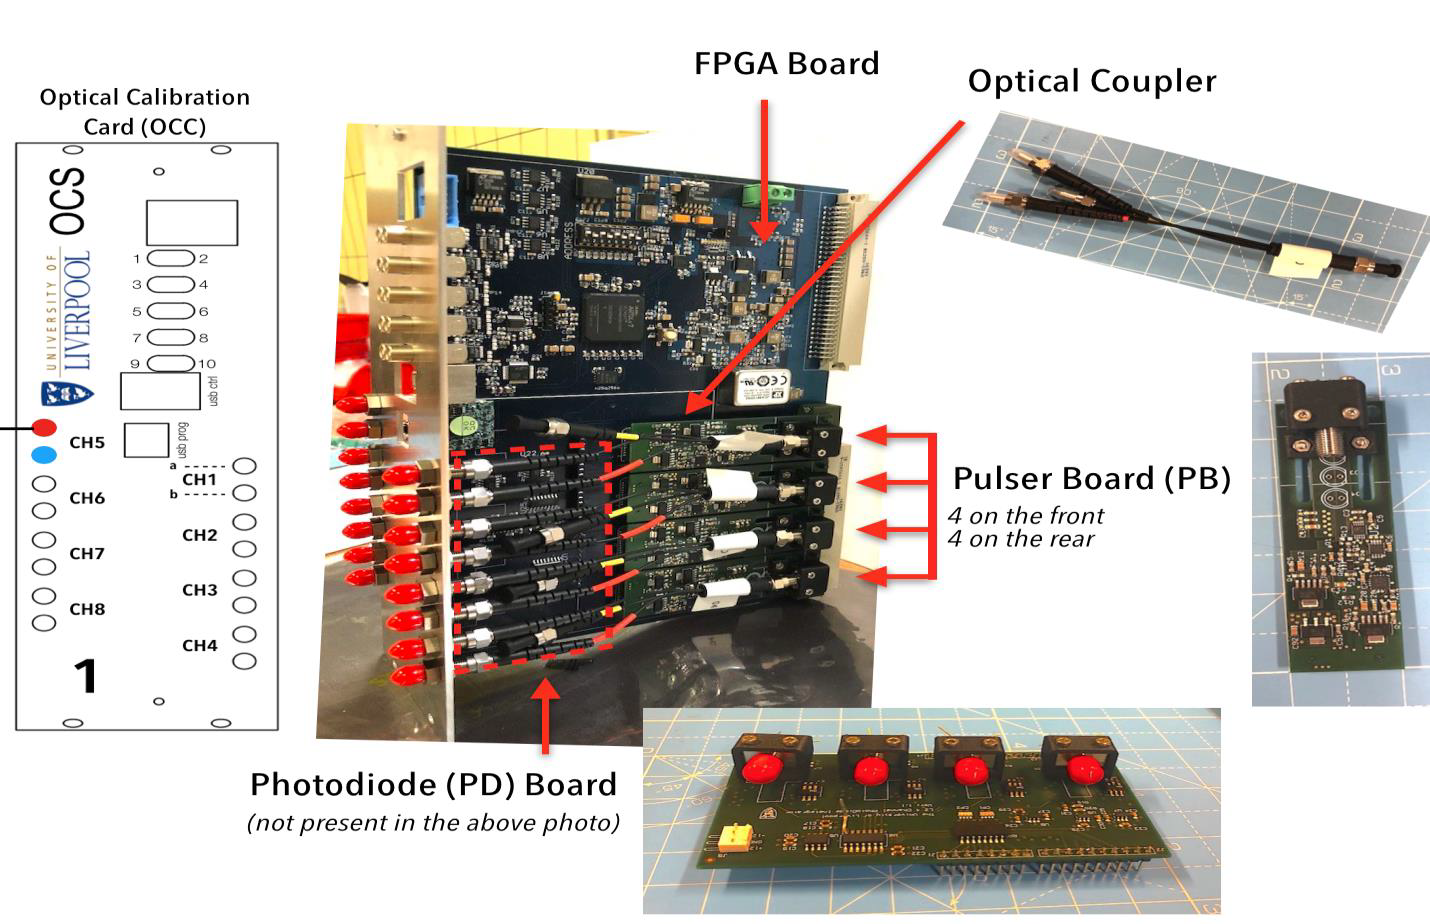
\includegraphics[width=\textwidth]{Figures/OCC.png}
    \caption{From left to right: a diagram of the front panel used on the OCC; a side profile of the FPGA motherboard with pulser boards, photo-diode board and optical couplers labelled respectively.}
    \label{fig:OCC}
\end{figure}

An optical calibration will be initiated by Run Control sending the required pulse configuration to Slow Control. Slow Control will store and manage the data needed to run a calibration. After each calibration run, collected data will be checked against previous calibration run data to ensure consistency of results between runs. The Slow Control system will run using the service, Ignition \cite{IgnitionWeb}, which will display data about the experiment running conditions, manage the database systems and control systems.
\newline
From Slow Control, control commands will pass to a BeagleBone X15 which will communicate with the FPGA boards setting the required registers. The BeagleBone will also read back board temperatures, photo-diode read back, pulse width and LED voltage to the Slow Control for real-time monitoring during calibration runs. A schematic of the OCS can be seen in figure \ref{fig:OCS_Flow}.  

\begin{figure}[ht]
    \centering
    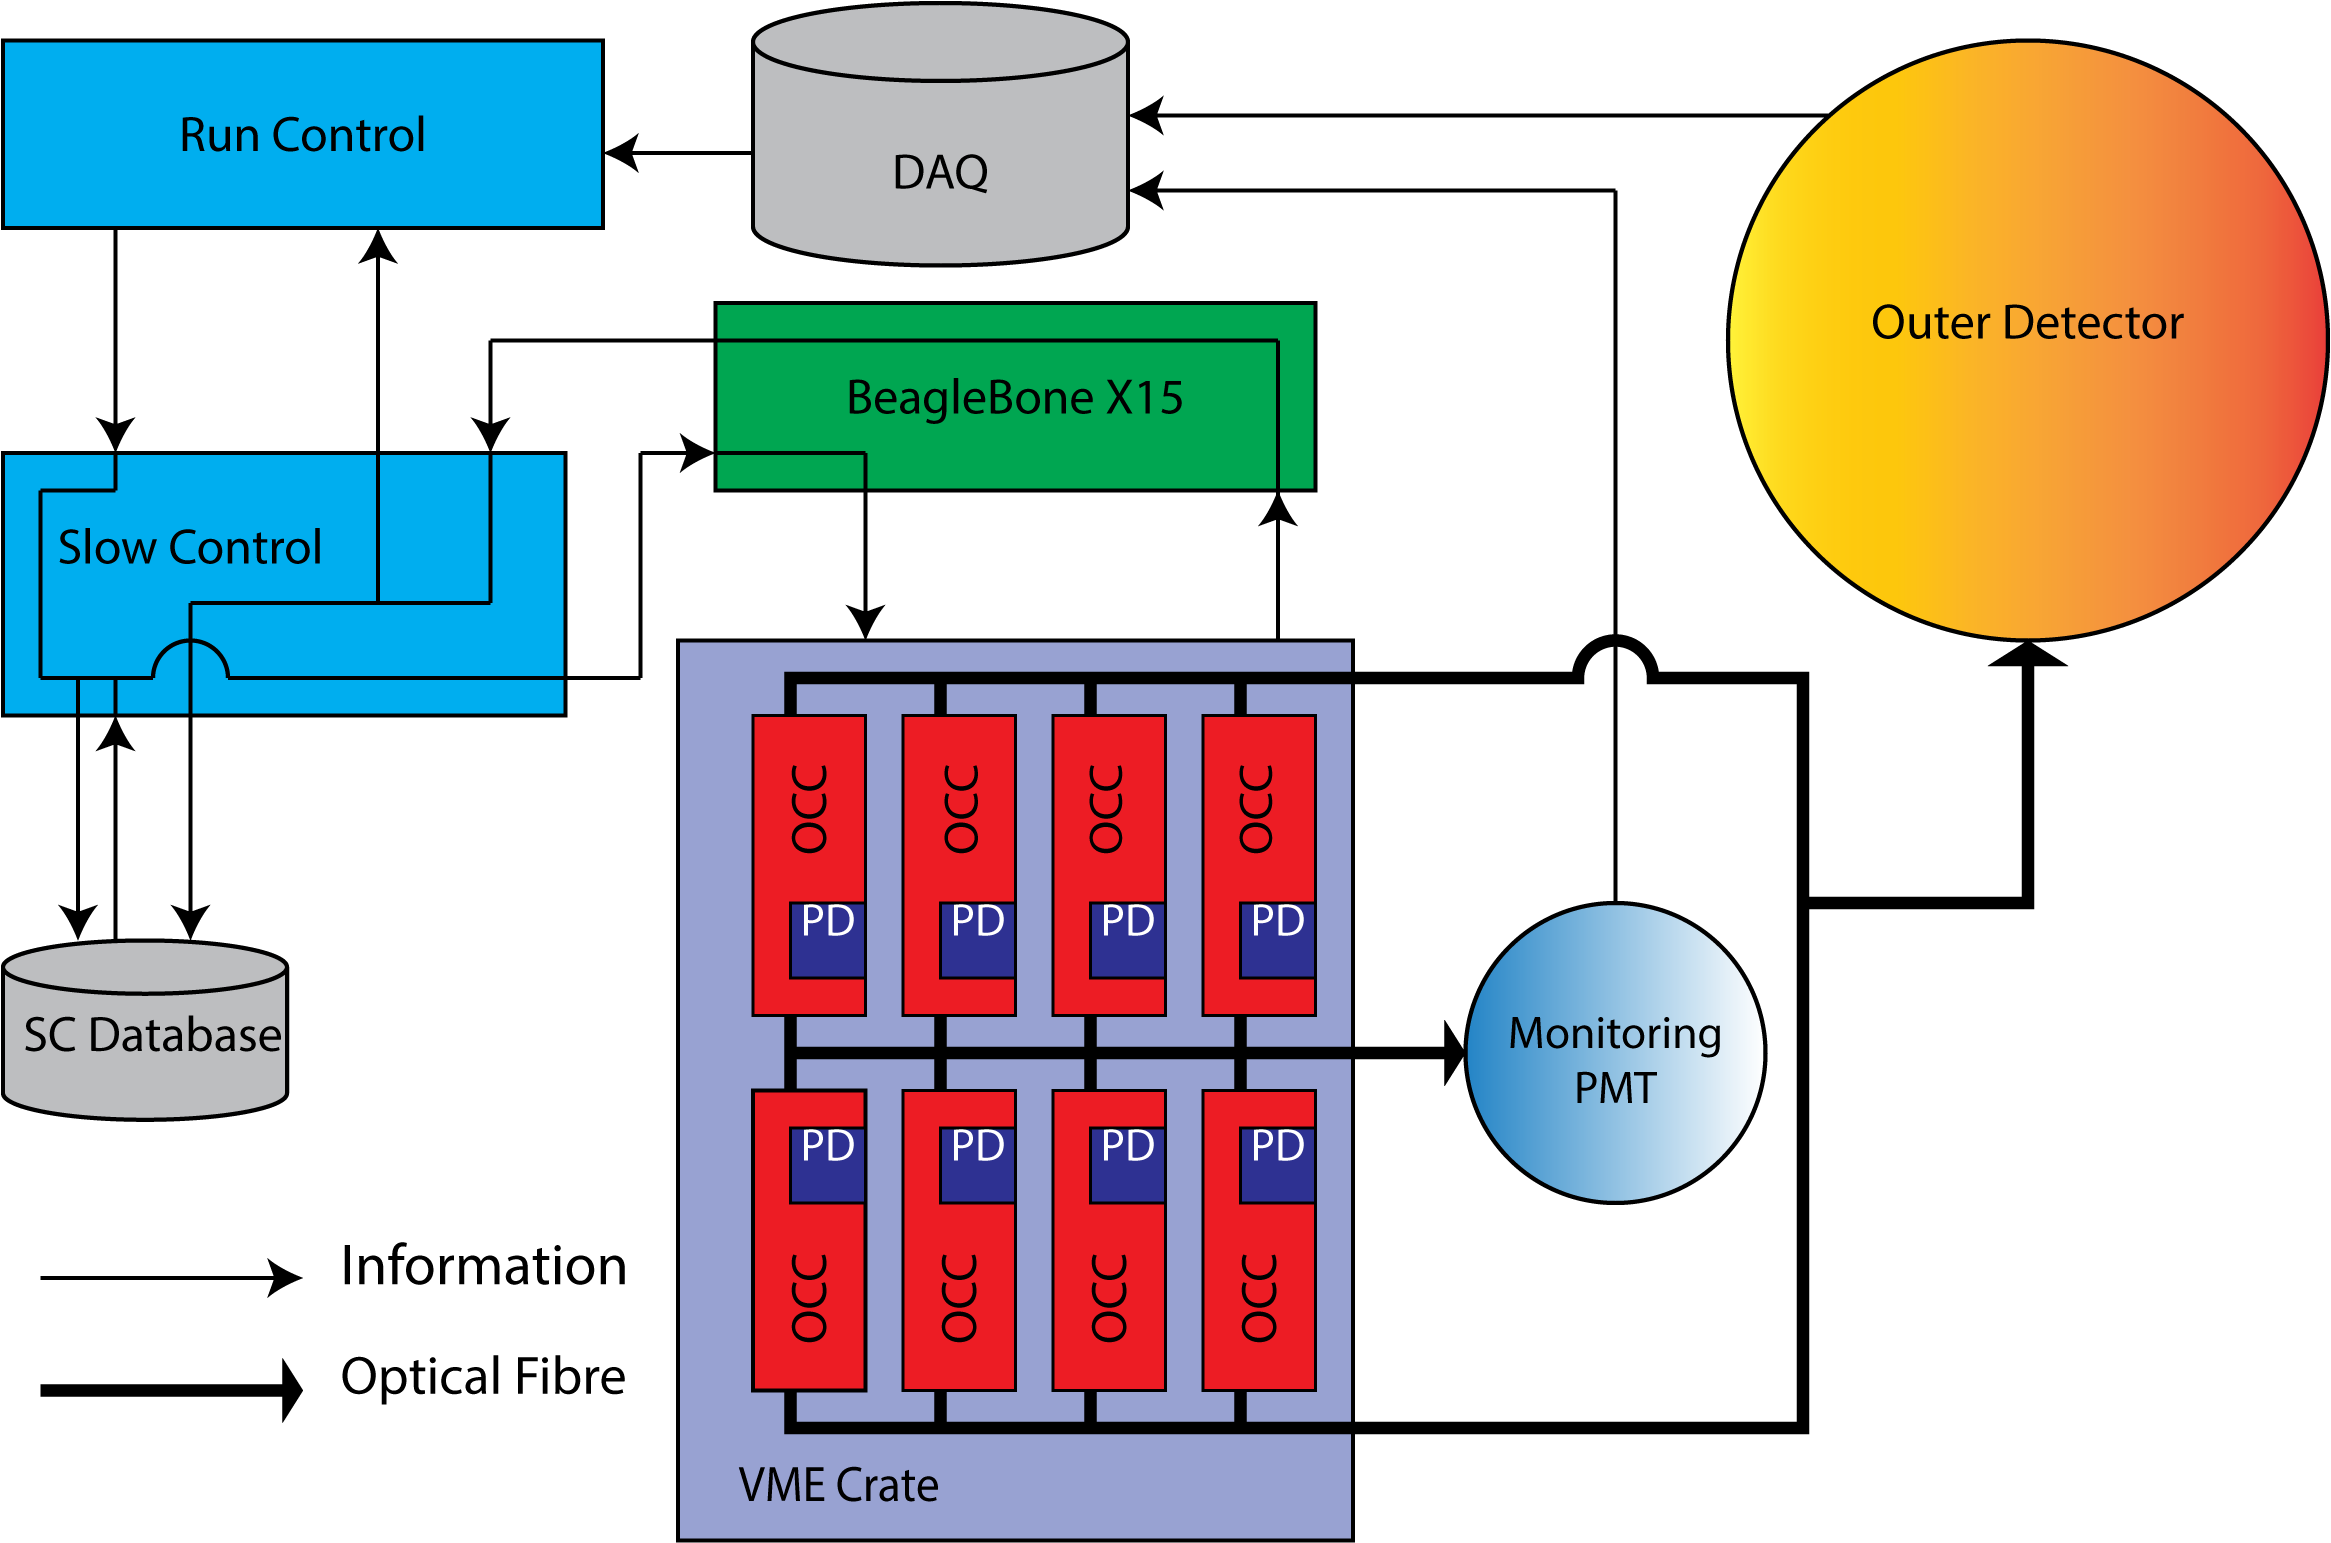
\includegraphics[width=\textwidth]{Figures/OCS.png}
    \caption{A schematic showing the working order in which an Outer Detector Optical Calibration will be completed: RC requests an Optical Calibration of the OD with the required pulse configuration; Slow Control analyses the received pulse configuration and retrieves specific parameters from the Slow Control-Database; Slow Control sends the specific parameters to a BeagleBone-X15; The BeagleBone-X15 communicates the specific commands to the VME Crate/OCCs setting the required registers; Light is pulsed into the OD and monitoring PMT; Readout from the monitoring PMT and OD is sent to the DAQ; Readouts from the photo-diode boards and OCCs are sent back to Slow Control-Database and Run Control via the BeagleBone-X15.}
    \label{fig:OCS_Flow}
\end{figure}

\chapter{OCC firmware update testing}\label{Chap7:FST}
The firmware to control the OCCs has been updated over the last year as data requirements have changed and the ability to use more precise timing increments have became available. Testing the updated firmware versions has been essential to confirm uniformity in the data collected between versions. In this section the testing procedure, firmware changes and results will be discussed.

\section{Full system test}
During each full system test (FST) the optical calibration cards are inserted into a VME crate and is connected to a computer via USB for control, as seen in figure \ref{fig:TestStand}. On the computer a python script is used to control the testing procedure. The process of testing is fully automated and initiated with the user inputting scan settings. The python scripts start the test with a given set pulse widths, pulse frequency and constants. The control commands and test settings are sent from the computer using a set of predefined registers to the OCC and interpreted by the FPGA motherboard. The FPGA chip controls the pulser board to pulse the light with pre-defined settings. The FPGA motherboard also sends the pulse width and pulse frequency to the oscilloscope for visual interpretation. Light from the pulser board is split down three optical fibres using an optical coupler. The first optical fibre is connected to a photo-diode board and the output is read back to the computer via the FPGA motherboard. The second optical fibre is connected to a power meter and this output is read back directly to the computer by USB. The third optical fibre is connected to a Hamamatsu H10721 PMT. The PMT is connected to the oscilloscope for visual interpretation. A DRS4 Evaluation Board is used to digitise the PMT pulses and FPGA board triggers at 5 Giga samples per second. Data from the DRS4 is read back directly to the computer by USB \cite{DRS4}. An Arudino board is used to control the gain of the PMT controlled from the python script. The test stand is setup such that only one channel can be tested at any one time. A schematic of the test stand can be seen in figure \ref{fig:FST_Flow}. The following list illustrates the data taken on each test:

\begin{itemize}\label{list:FSTdata}
    \item Number of photons per pulse with error
    \item Time on system clock
    \item Trigger width
    \item Trigger amplitude
    \item Position of the trigger peak
    \item Pulse width
    \item Pulse amplitude
    \item Position of pulse peak
    \item Width set
\end{itemize}

\begin{figure}[h]
    \centering
    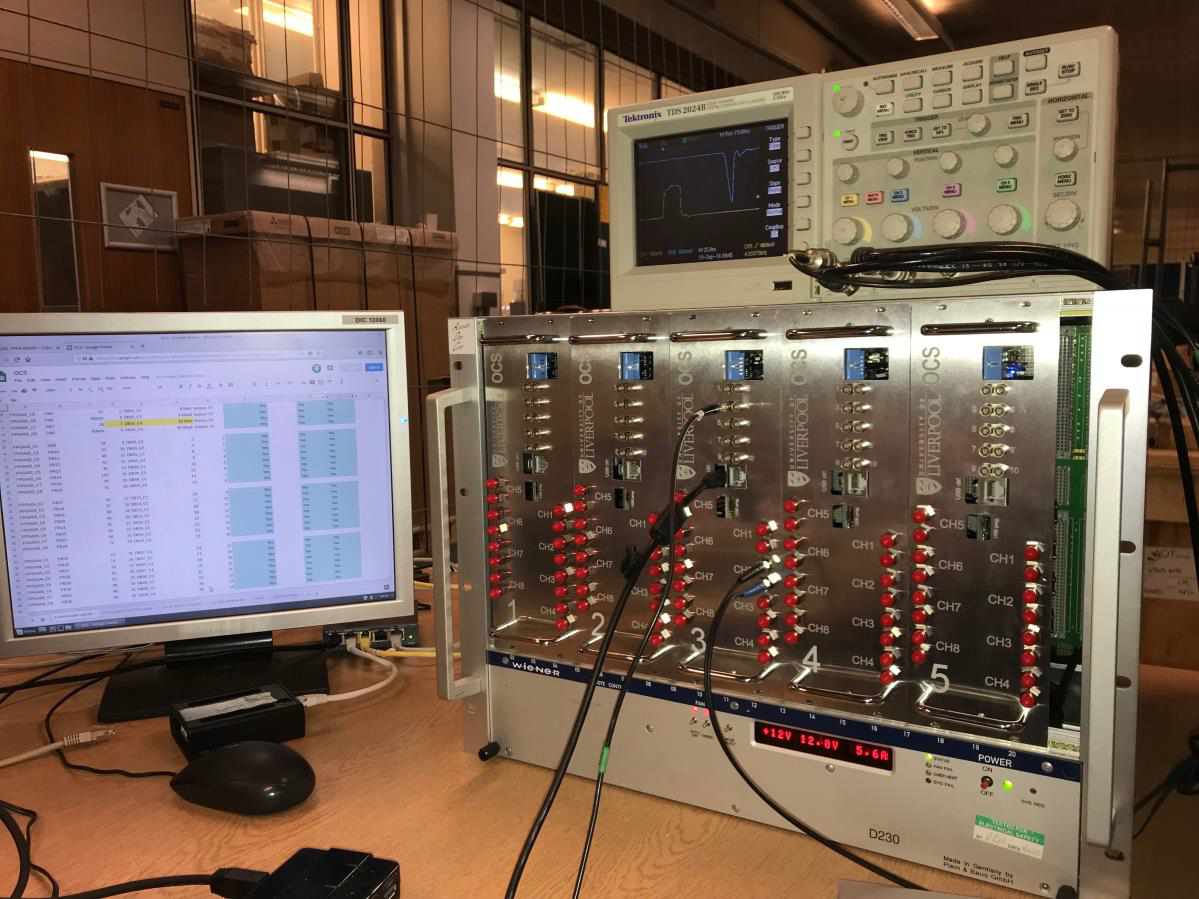
\includegraphics[width=0.7\textwidth]{Figures/TestStand.png}
    \caption{Test stand with the OCCs placed in the VME crate and oscilloscope connected for testing.}
    \label{fig:TestStand}
\end{figure}

\begin{figure}[h!]
    \centering
    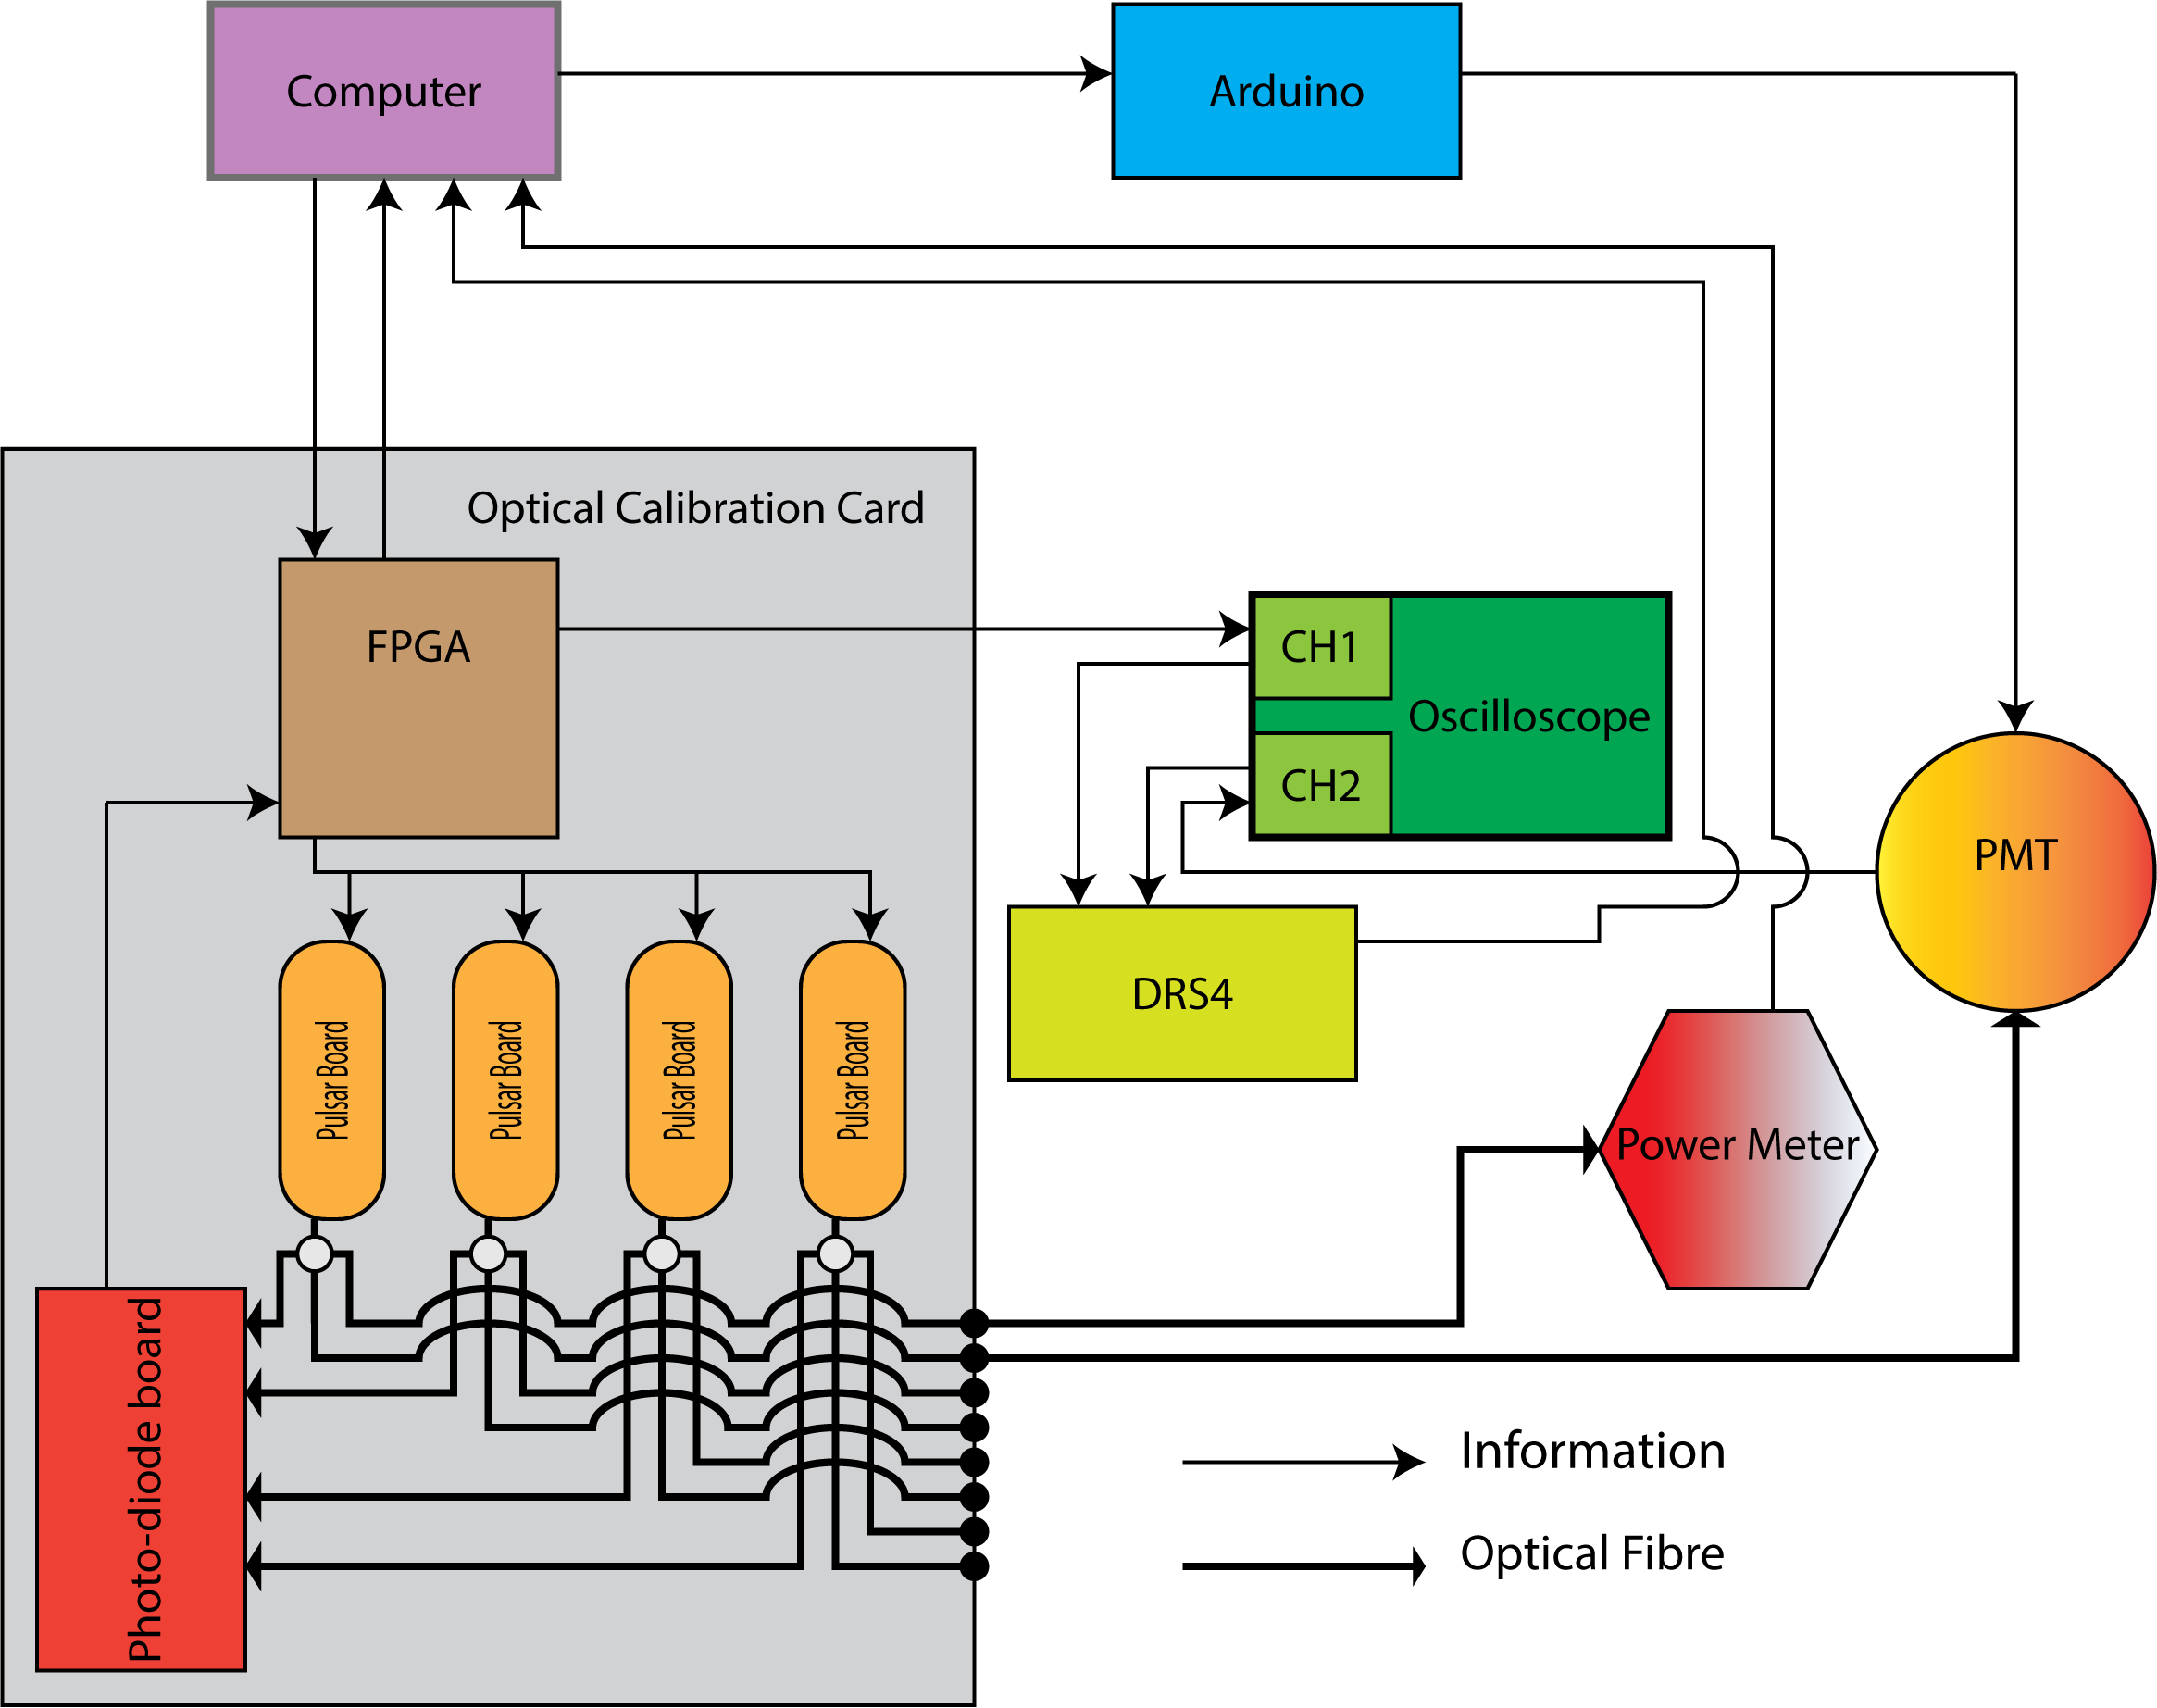
\includegraphics[width=0.7\textwidth]{Figures/FST.png}
    \caption{Schematic of the FST on a channel by channel test schedule. One board has been shown to demonstrate the process, showing the front side on an OCC. The remaining pulser boards and photo-diode board are located on the rear of the OCC.}
    \label{fig:FST_Flow}
\end{figure}

\section{Results}
After each OCC firmware update a full system test was conducted to confirm that the changes made to the firmware work correctly and to check the uniformity between firmware versions. Only one OCC was used throughout the testing as the firmware was updated, this decision was made due to time constraints. The data sets which were checked between firmware updates are: trigger width; pulse width; and width set. These data sets were monitored due to the changes which were made in the firmware. The data presented in the following subsections is from tests conducted on OCC-2 Channel 2 corresponding to pulser board 10.
\subsection{Trigger width}\label{subsec:trigw}
The Trigger Width (TW) is the measured width of the electronic pulse which is sent to the pulser board in order to produce light from the LED. TW is plotted against the natural logarithm of the number of photons per pulse (lnNph) in figure \ref{fig:trigw}. Figures \ref{fig:trig1},\ref{fig:trig2} and \ref{fig:trig3} have been fitted with the equation \ref{eqn:trigfit} where A, B and C correspond to calibration coefficients.  
\begin{equation}
    TW = A + e^{Bln(Nph)^2 + Cln(Nph))}
\label{eqn:trigfit}
\end{equation}
The optical calibration program will utilise equation \ref{eqn:trigfit} to determine the trigger width needed when a user defines the number of photons to inject into the OD. Equation \ref{eqn:trigfit} is currently being adapted to fit to the more complex curve produced by the data seen in figure \ref{fig:trig4}. In firmware version 1 and version 2, a $\sim5ns$ step in trigger width was used for faster testing capabilities in early tests. In firmware version 3 and version 4, a $\sim75ps$ step in the trigger width was implemented, utilising the full capability of the FPGA motherboard. Decreasing the step in trigger width measurements allows for more data points within the given trigger width range, this results in a fit function which represents the data more precisely. 
\newline
The equation fitted to the data has not been developed throughout the firmware updates. As the number of data points has increased the equation will be developed to reduce the $\chi^2$ value associated with the fit. 
\newline
As discussed early, the fit function will be used in the OCS to determine the trigger width corresponding to a specific number of photons, so the accuracy of the function is paramount. 

\begin{figure}[ht!]
\centering
    \begin{subfigure}[b]{.475\textwidth}
        \centering
        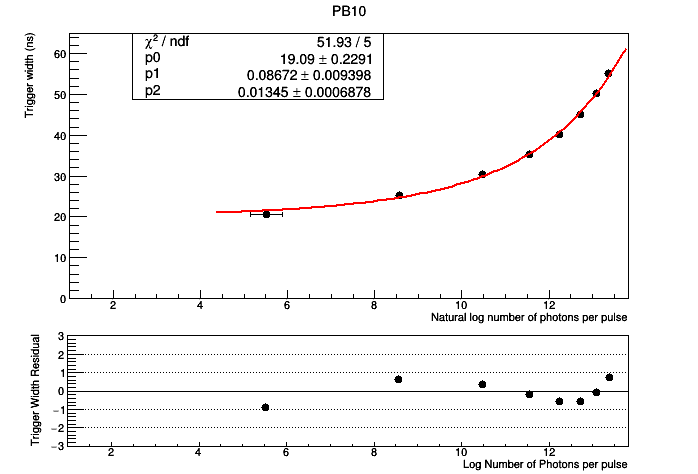
\includegraphics[width=\textwidth]{Figures/Plots/V1_ln(Nph)vsTriggerWidthResidual.png}
        \caption{Firmware version 1.}
        \label{fig:trig1}
    \end{subfigure}
    \hfill
    \begin{subfigure}[b]{.475\textwidth}
        \centering
        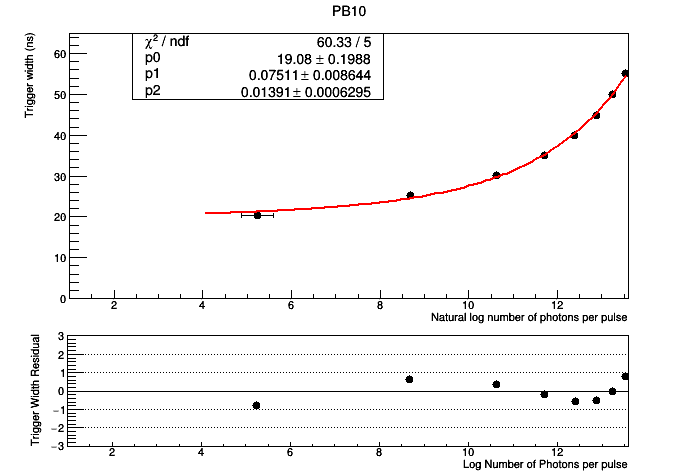
\includegraphics[width=\textwidth]{Figures/Plots/V2_ln(Nph)vsTriggerWidthResidual.png}
        \caption{Firmware version 2.}
        \label{fig:trig2}
    \end{subfigure}
    \vskip\baselineskip
    \begin{subfigure}[b]{.475\textwidth}
        \centering
        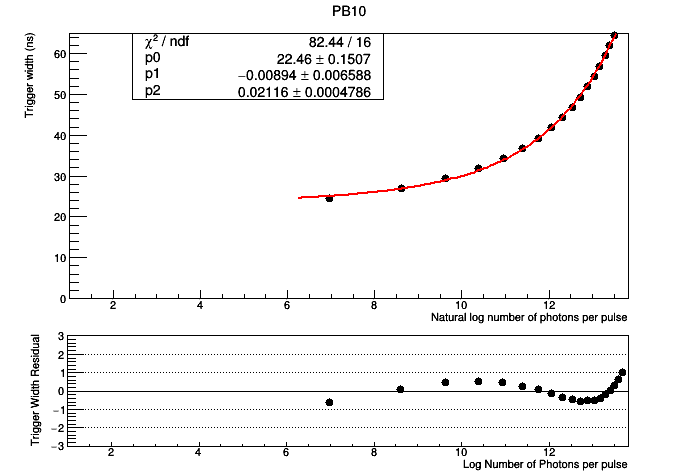
\includegraphics[width=\textwidth]{Figures/Plots/V3_ln(Nph)vsTriggerWidthResidual.png}
        \caption{Firmware version 3.}
        \label{fig:trig3}
    \end{subfigure}
    \hfill
    \begin{subfigure}[b]{.475\textwidth}
        \centering
        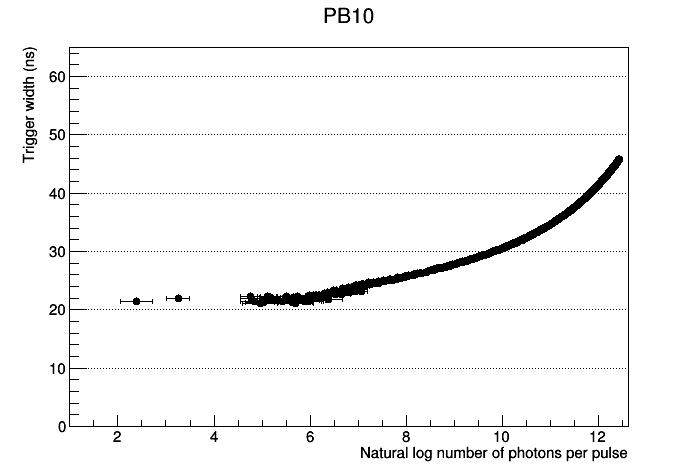
\includegraphics[width=\textwidth]{Figures/Plots/V4_ln(Nph)VSTriggerWidthPB10.png}
        \caption{Firmware version 4.}
        \label{fig:trig4}
    \end{subfigure}
    \caption{The evolution of the trigger widths measured as the OCC firmware was updated. The natural logarithm of the number of photons per pulse was used to aid the fitting the calibration curve to the plot. The fit residual is plotted below each plot where the data has been fitted with the equation \ref{eqn:trigfit}.}
    \label{fig:trigw}
\end{figure}



\subsection{Pulse width}\label{subsec:pulsew}
The Pulse Width is the measured taking the full width at half peak maximum of the light pulse which is detected by the PMT. Pulse width is monitored between firmware versions to ensure the system meets the requirements set by LZ (\ref{list:SystemReq}). Pulse Width is plotted against the logarithm of the number of photons per pulse in figure \ref{fig:trigw}.  
\begin{figure}[ht!]
\centering
    \begin{subfigure}[b]{.475\textwidth}
        \centering
        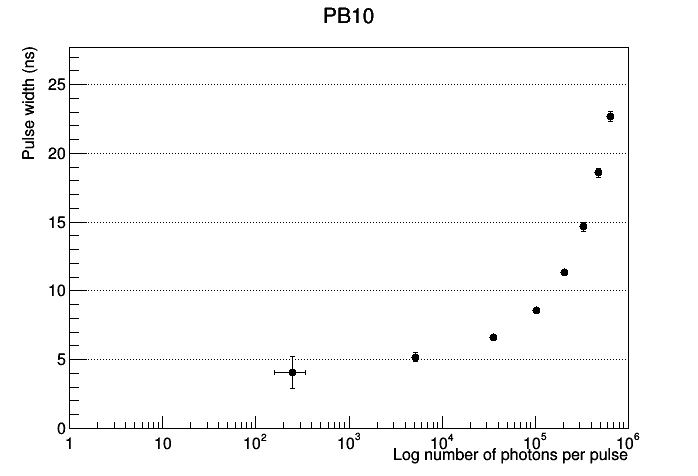
\includegraphics[width=\textwidth]{Figures/Plots/V1_log(Nph)vsPulseWidthPB10.png}
        \caption{Firmware version 1.}
        \label{fig:pulse1}
    \end{subfigure}
    \hfill
    \begin{subfigure}[b]{.475\textwidth}
        \centering
        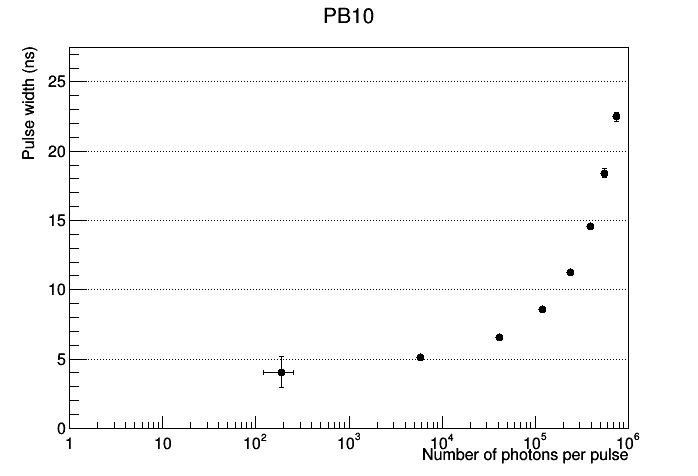
\includegraphics[width=\textwidth]{Figures/Plots/V2_log(Nph)vsPulseWidthPB10.png}
        \caption{Firmware version 2.}
        \label{fig:pulse2}
    \end{subfigure}
    \vskip\baselineskip
    \begin{subfigure}[b]{.475\textwidth}
        \centering
        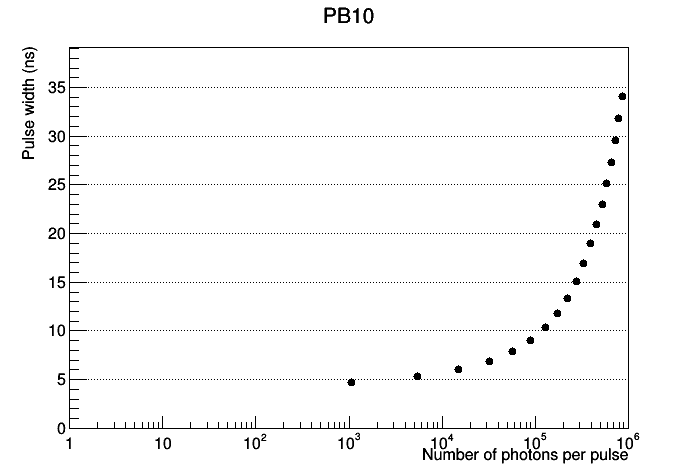
\includegraphics[width=\textwidth]{Figures/Plots/V3_log(Nph)vsPulseWidthPB10.png}
        \caption{Firmware version 3.}
        \label{fig:pulse3}
    \end{subfigure}
    \hfill
    \begin{subfigure}[b]{.475\textwidth}
        \centering
        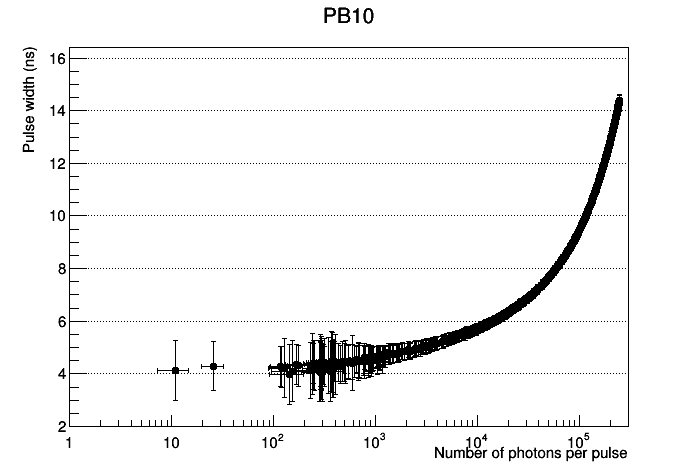
\includegraphics[width=\textwidth]{Figures/Plots/V4_log(Nph)VSPulseWidthPB10.png}
        \caption{Firmware version 4.}
        \label{fig:pulse4}
    \end{subfigure}
    \caption{Evolution of the pulse widths measured as the OCC firmware was updated. The logarithm of the number of photons per pulse is plotted against the pulse width.}
    \label{fig:pulsew}
\end{figure}
\subsection{Width set}\label{subsec:widthset}
The width set values correspond to scan points throughout the testing. As discussed in subsection \ref{subsec:trigw}, in firmware versions 1 and 2 a trigger width step of $\sim5ns$ was implemented resulting in the testing of 8 scan points. In testing firmware version 3, 19 points were scanned. In firmware version 4, 640 points were scanned. The increase in scan points between versions was due to the change in trigger width step. In firmware version 4, 10 large width set points were used with each large width set step containing 64 small width set points. Width set was monitored between firmware versions as the values used for iteration within scripts to produced the plots in figures \ref{fig:trigw},\ref{fig:pulsew} and \ref{fig:widthset}.
\begin{figure}[ht!]
\centering
    \begin{subfigure}[b]{.475\linewidth}
        \centering
        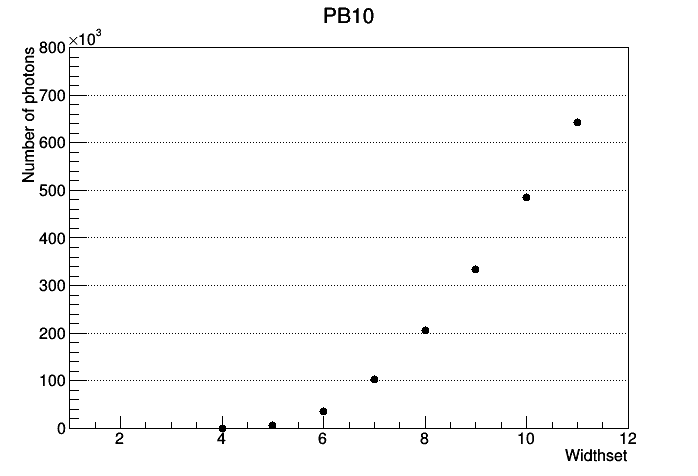
\includegraphics[width=\textwidth]{Figures/Plots/V1_widthsetVSNphPB10.png}
        \caption{Firmware version 1.}
        \label{fig:width1}
    \end{subfigure}
    \hfill
    \begin{subfigure}[b]{.475\linewidth}
        \centering
        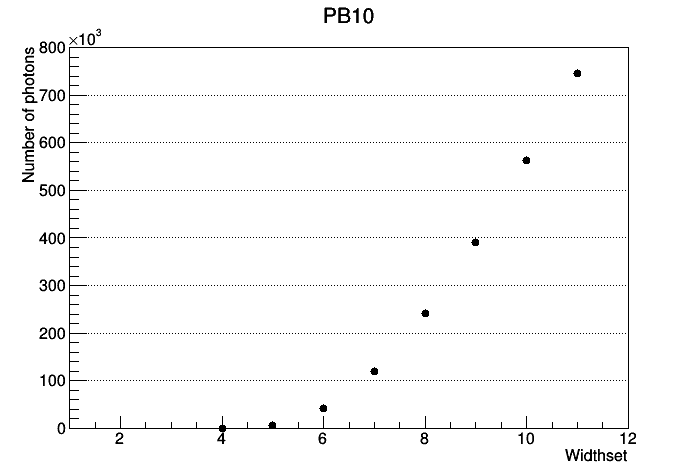
\includegraphics[width=\textwidth]{Figures/Plots/V2_widthsetVSNphPB10.png}
        \caption{Firmware version 2.}
        \label{fig:width2}
    \end{subfigure}
    \vskip\baselineskip
    \begin{subfigure}[b]{.475\linewidth}
        \centering
        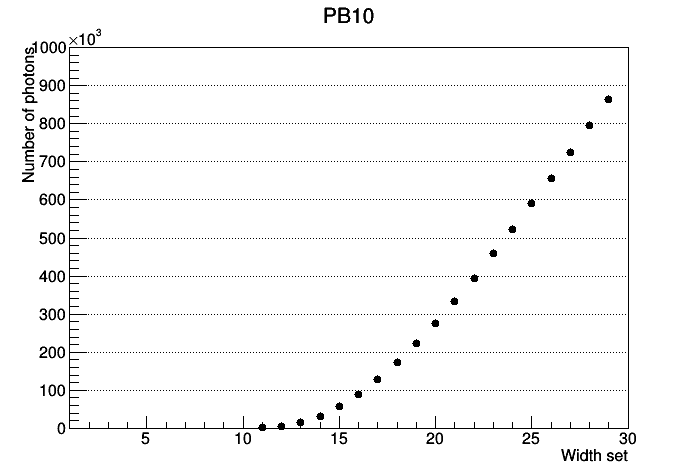
\includegraphics[width=\textwidth]{Figures/Plots/V3_widthsetVSNphPB10.png}
        \caption{Firmware version 3.}
        \label{fig:width3}
    \end{subfigure}
    \hfill
    \begin{subfigure}[b]{.475\linewidth}
        \centering
        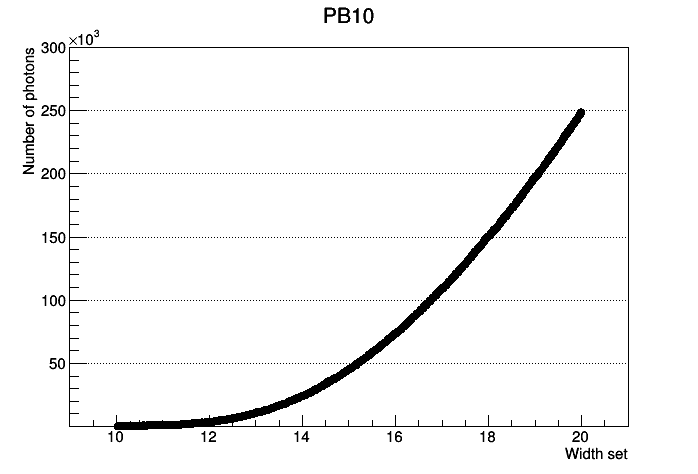
\includegraphics[width=\textwidth]{Figures/Plots/V4_widthsetVSNphPB10.png}
        \caption{Firmware version 4.}
        \label{fig:width4}
    \end{subfigure}
    \caption{Evolution of the width set used in the firmware updates. The number of photons per pulse is plotted against the width set.}
    \label{fig:widthset}
\end{figure}
\newline
The results obtained from the full system tests will be key in the development of the optical calibration program and will provide a suitable comparison when the system is installed.

\chapter{Fibre Support Structures}\label{Chap8:FSS}
At each light injection point the duplex optical fibre will be held in place using a Fibre Support Structure (FSS). The purpose of the FSS is to ensure each fibre is aligned correctly as it points in towards the scintillator tanks and to provide a consistent 50mm curvature of the duplex optical fibre. Each FSS consists of 26 parts: 7 machined PTFE structural components; 7 passivated bolts; 9 passivated inserts; and two PTFE inserts. A photograph of a FSS with the lid open can be seen in figure \ref{fig:FFS}.

\begin{figure}[h]
    \centering
    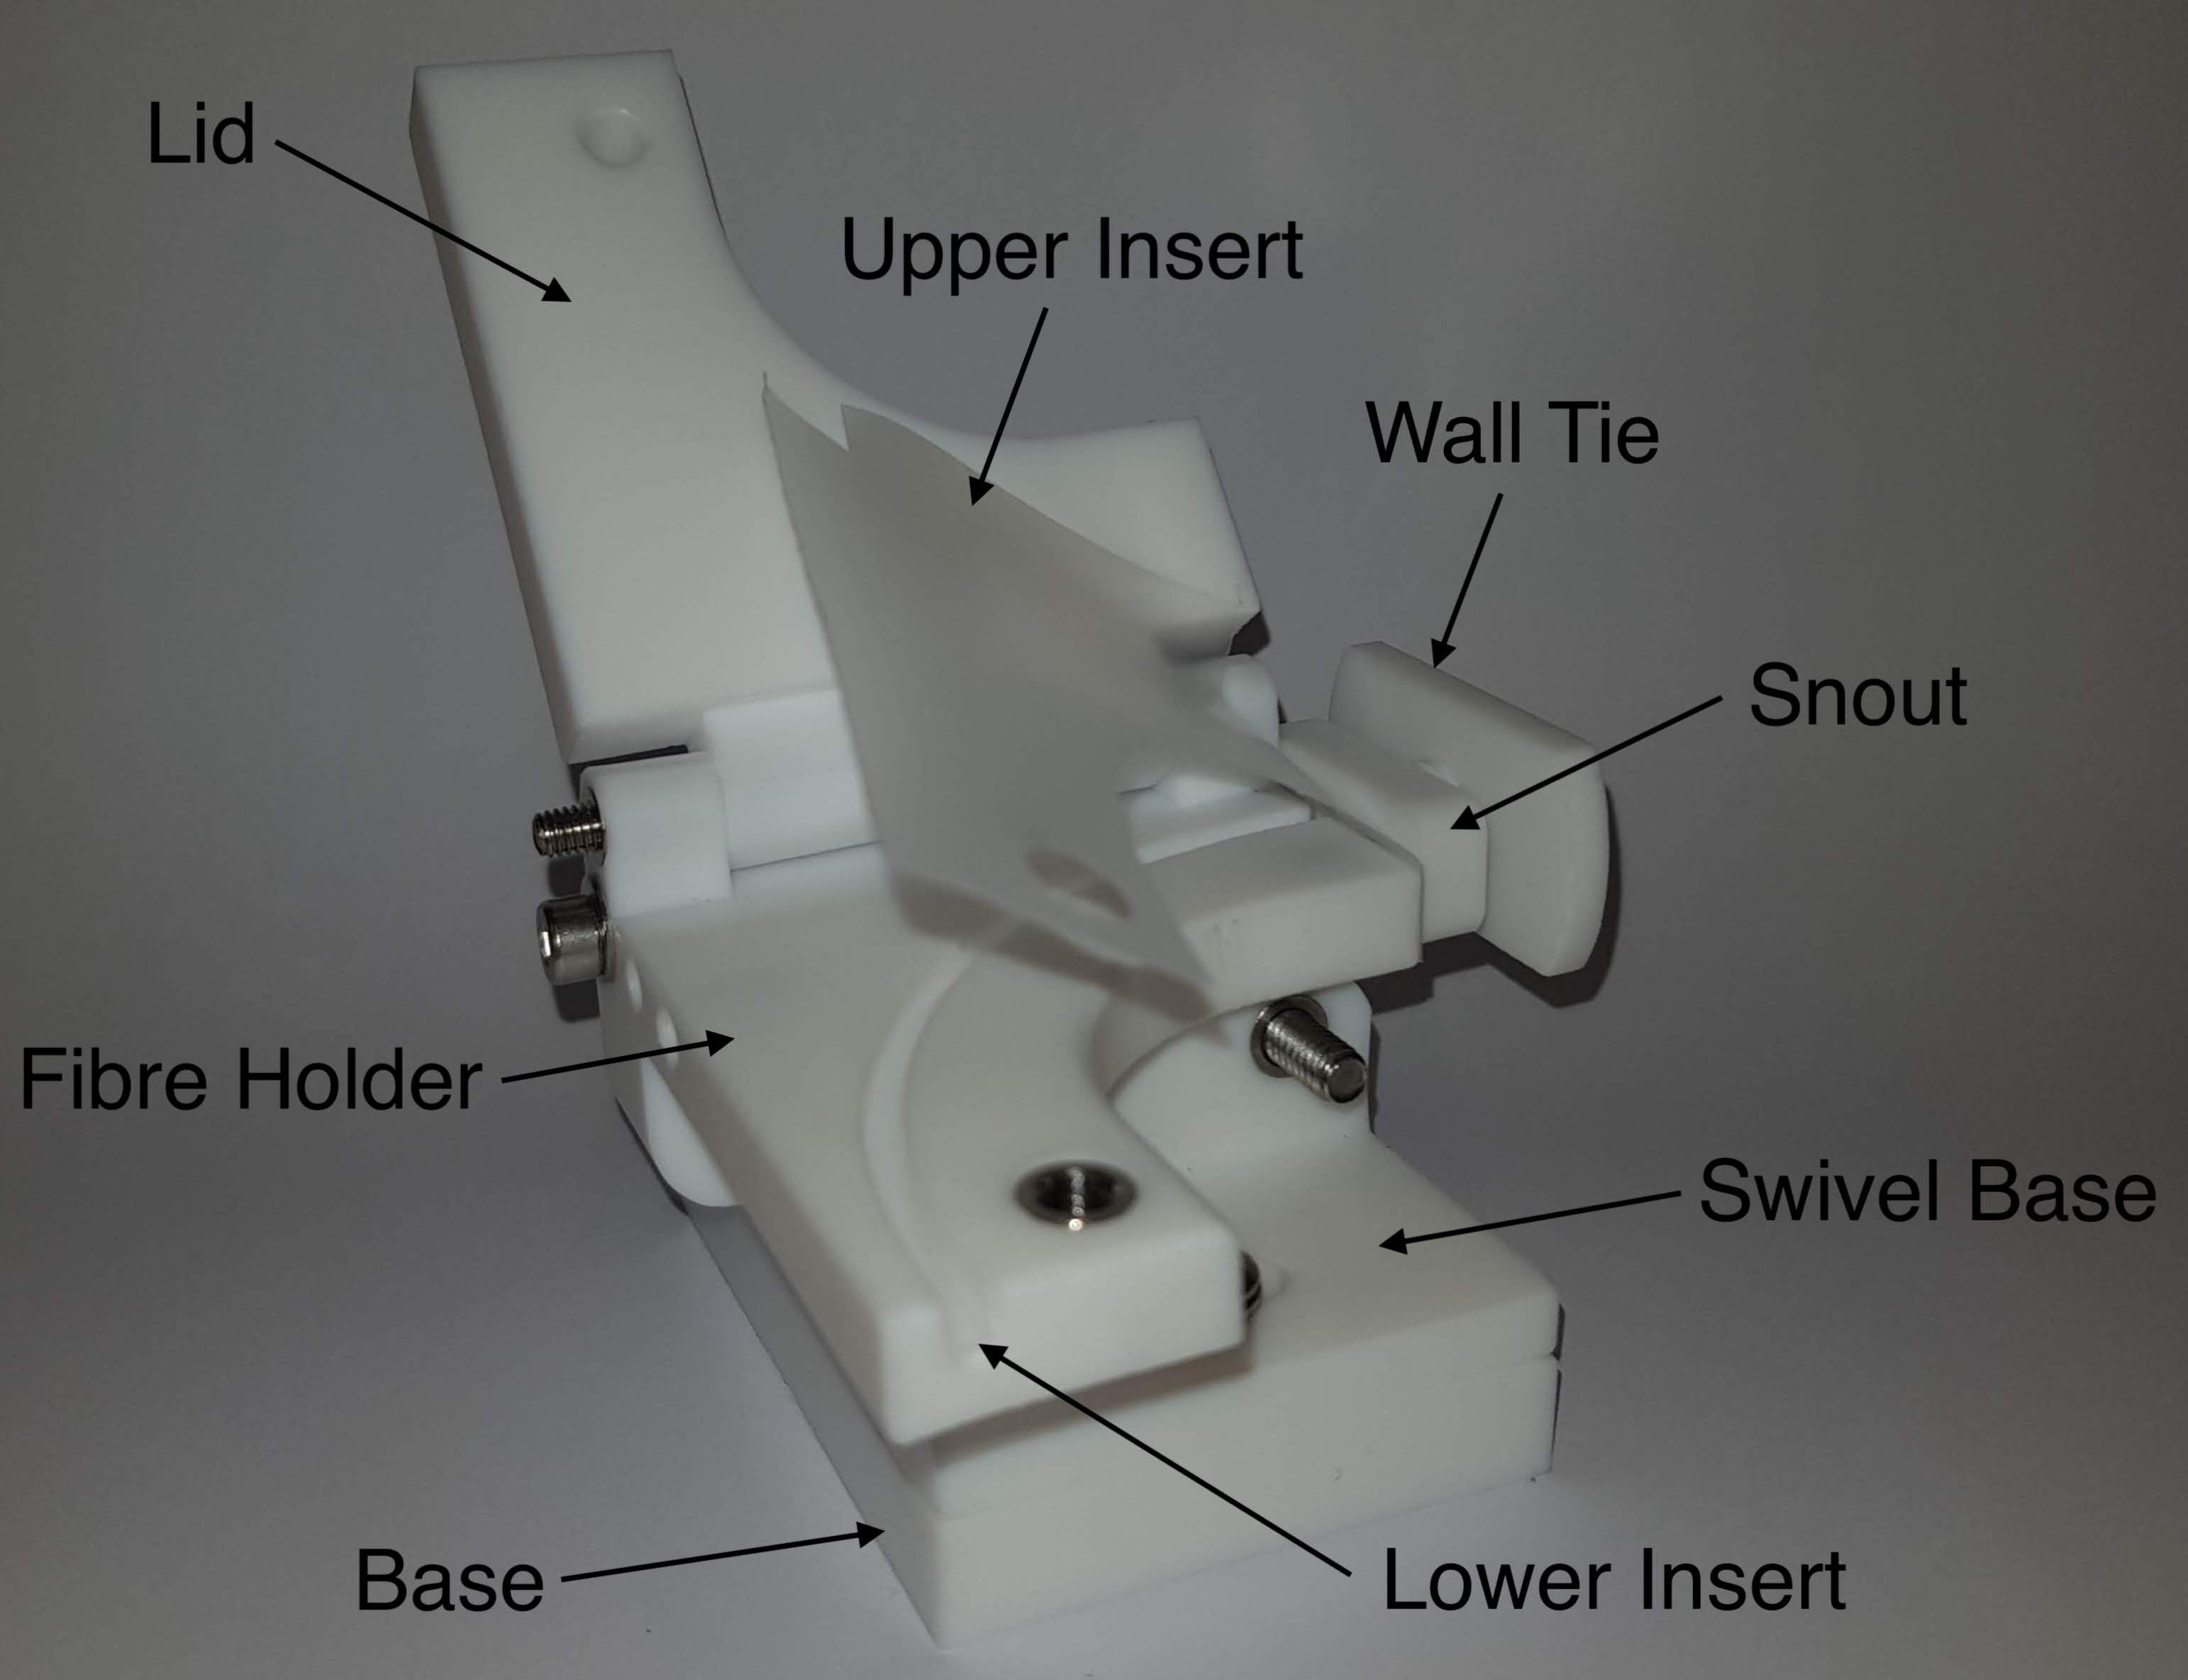
\includegraphics[width=0.7\textwidth, angle=0]{Figures/FSS.jpg}
    \caption{A photograph of one of the FSS with the lid open. The 8 key components of the FSS are labelled repectively}
    \label{fig:FFS}
\end{figure}

\section{Testing}
After the manufacturing of the FSS's was completed a random selection of 6 FSS's were sent to the Boulby Underground Laboratory for radioactive screening. The results from the screening have been compared to the estimated activities of the OD components in table \ref{table:radio-nuc}.  
\begin{table}[h!]
\centering
\begin{tabular}{|c|c|c|c|c|c|c|c|} 
    \hline
    Outer Detector Components & Mass / kg & $U_e^{238}$ & $U_l^{238}$ & $Th_e^{232}$ & $Th_l^{232}$ & $Co^{60}$ & $K^{40}$ \\
    & & \multicolumn{6}{c|}{Activity (mBq/kg)} \\
    \hline
    Outer Detector Tanks & 3200 & 0.16 & 0.39 & 0.02 & 0.06 & 0.04 & 5.36 \\
    \hline
    Liquid Scintillator & 17600 & 0.01 & 0.01 & 0.01 & 0.01 & 0.00 & 0.00 \\
    \hline
    Outer Detector PMTs & 205 & 570 & 470 & 395 & 388 & 0.00 & 534 \\
    \hline
    OD PMT Supports & 770 & 1.20 & 0.27 & 0.33 & 0.49 & 1.60 & 0.40 \\
    \hline
    Fibre Support Structure & 0.350 & 31 & 3.0 & 6.0 & 3.0 & 0.5 & 330 \\
    \hline
\end{tabular}
\caption{Estimated activities of the radio-nuclides present in the OD components are presented with the results from the screening of the FSSs at Boulby Underground Laboratory. A comprehensive list of the estimated activities for the rest of the detector can be found in the LZ-TDR \cite{LZTDR}.}
\label{table:radio-nuc}
\end{table}
In comparison with the OD components, the results show relatively large activities in potassium-40 in the screened sample. This could be due to environmental containment's which remained on the sample after being wiped with propan-2-ol. Before the next set of samples are sent for screening, they will be cleaned using the procedure that will be implemented before installation at the experiment. Results from the two screenings will be compared to ensure that the high levels of potassium-40 is due to environmental containment's and not from containment's within the PTFE material.

\section{Fibre support structure - insert development}\label{sec:FSSID}
After the construction a duplex optical fibre was place into the FSS and it was found that the PTFE material which the structural components were produced from didn't grip the fibre when a small force was applied. In this section, the series of tests and the components produced to resolve this problem will be discussed. 

\subsection{Insert description}
Two inserts were designed to fit between the fibre and the PTFE material. The templates for the inserts can be seen in figure \ref{fig:inserts}. The upper insert is placed in groove of the fibre holder below the fibre and lower insert is placed between the lid of the FFS and the fibre holder component, seen in figure \ref{fig:FFS}. Both inserts are attached to the FSS using bolts which are used to attach the snout piece to the fibre holder.

\begin{figure}[h!]
    \centering
    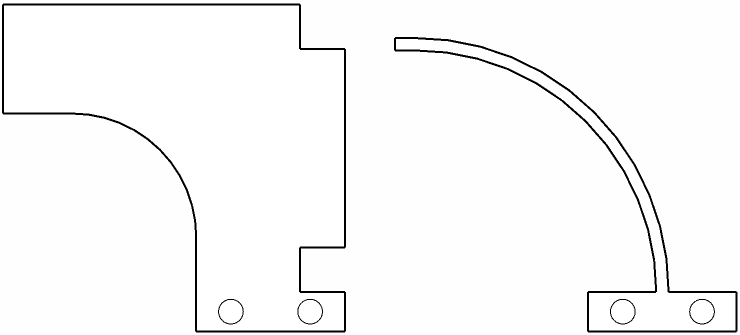
\includegraphics[width=0.7\textwidth]{Figures/Slip_inserts.jpg}
    \caption{Inserts are designed to fit between the duplex fibre and the PTFE components of the FSS. The upper insert is placed between the FSS lid and the fibre (left). The lower insert is placed between the fibre and FSS fibre holder, sitting inside the groove (right).}
    \label{fig:inserts}
\end{figure}

\subsection{Testing}
The force required to induce creep in the fibre when being held by the FSS was tested using the apparatus in figure \ref{fig:FPTT_Test_Stand}. Variations in the arrangement of the inserts were tested in varying moisture conditions. The arrangements tested were: no inserts (A); one upper insert with no lower insert (B); two upper inserts with no lower insert (C); and one upper insert with one lower insert (D). The moisture conditions were varied between: "dry" where no water was used; "drip" where de-ionised water was pipetted down the groove of the fibre holder; and "submersion" where the entire FSS was submerged in de-ionised water to simulate how the FSS would perform in the water tank of the OD. Each of the insert arrangements were tested under dry conditions and then the best two were tested under more moist conditions. The results from the testing can be found in table \ref{table:FPTT} and are displayed in figure \ref{fig:FPTT_plot}. 

\subsection{Results}
In the test arrangement D performed best in comparison with the other arrangements under the varied moisture conditions and it would be recommended that this arrangement is used during the running of the experiment. It can also be seen that the force required to pull the fibre from the FSS should be greater than any force encountered on the fibres. 

\begin{figure}[h]
    \centering
    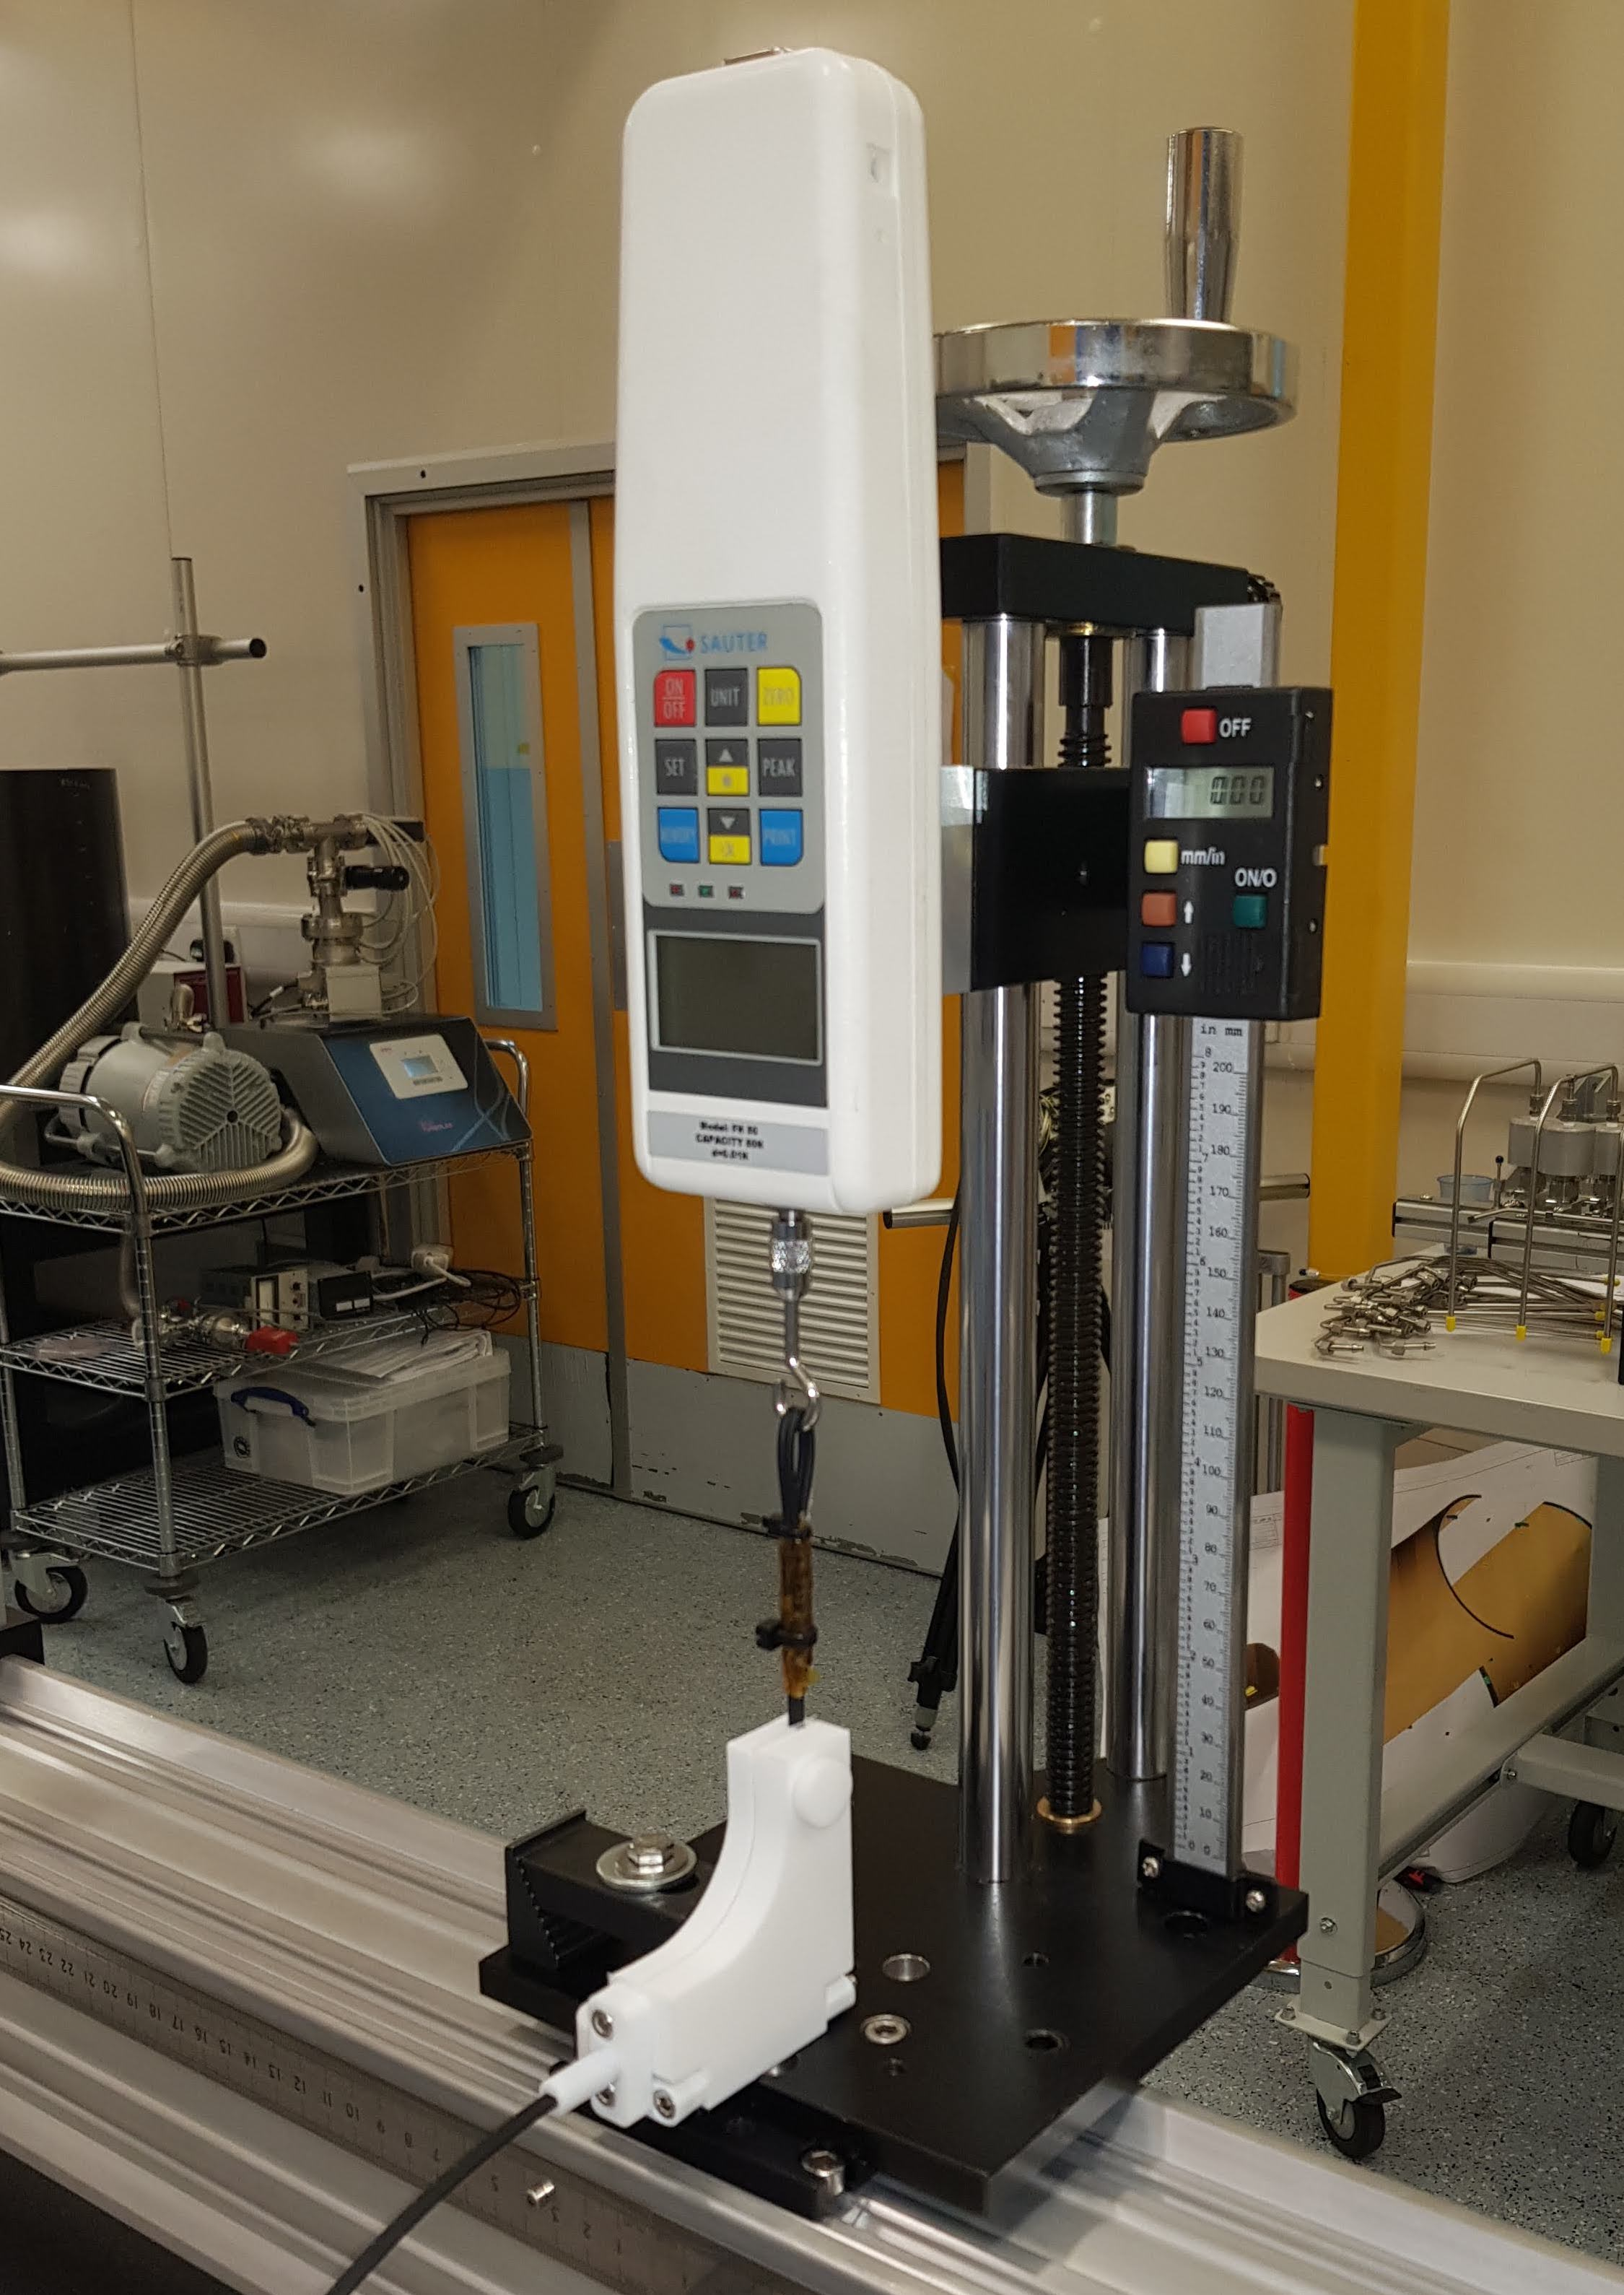
\includegraphics[width=0.6\textwidth]{Figures/FPTT_Test_Stand.jpg}
    \caption{Photograph showing the setup of the apparatus used in the fibre pull through test.}
    \label{fig:FPTT_Test_Stand}
\end{figure}

\begin{table}[h!]
\centering
    \begin{tabular}{c|c|c|c|} 
        \cline{2-4}
        & \multicolumn{3}{|c|}{Moisture Condition}
        \cr. \cline{2-4}
        \hline
        \multicolumn{1}{|c|}{Insert Arrangement} &Dry / N& Drip / N& Submersion / N\\
        \hline
        \multicolumn{1}{|c|}{A} & $6.4 \pm 0.2$ & - & - \\
        \multicolumn{1}{|c|}{B} & $12.0 \pm 0.3$ & - & - \\
        \multicolumn{1}{|c|}{C} & $13.4 \pm 0.5$ & $12.0 \pm 0.3$ & - \\
        \multicolumn{1}{|c|}{D} & $17.8 \pm 1.1$ & $18.4 \pm 1.1$ & $16.4 \pm 0.3$ \\
        \hline
    \end{tabular}
\caption{In this table, the force required to induce creep in the fibre under varying moisture conditions and insert arrangement.}
\label{table:FPTT}
\end{table}

\begin{figure}[h]
    \centering
    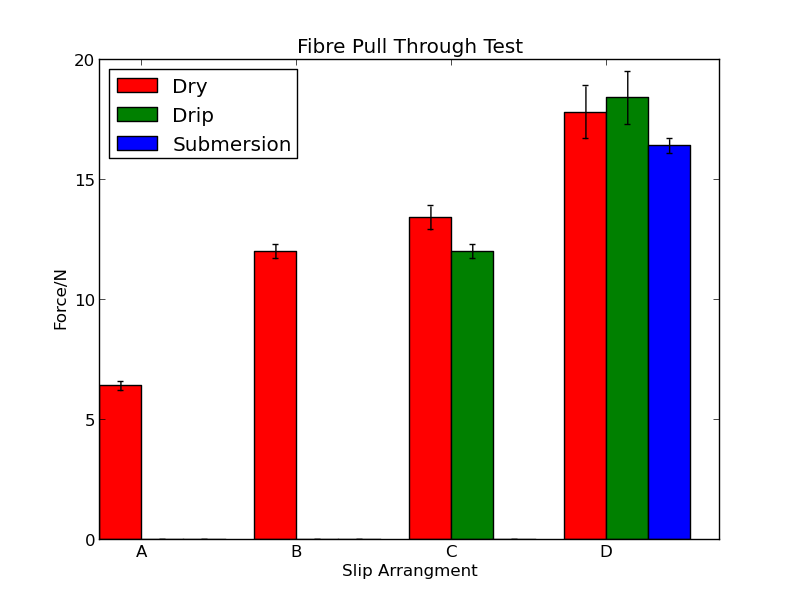
\includegraphics[width=0.7\textwidth]{Figures/FPTT_plot.png}
    \caption{Plot showing the force required to move a fibre under varied moisture conditions with different slip arrangements.}
    \label{fig:FPTT_plot}
\end{figure}

In the test arrangement D performed best in comparison with the other arrangements under the varied moisture conditions and it would be recommended that this arrangement is used during the running of the experiment. It can also be seen that the force required to pull the fibre from the FSS will be greater than any force which could be generated from waves oscillating during the filling of the water tank. 


\chapter{Discussion and future work}\label{Chap10:Discussion}
In this first year report, a successful review of the cosmological indications for Dark Matter (\S\ref{Chap2:Cosmo}) and the possible candidates (\S\ref{Chap3:Candi}) preceded a description of the possible methods in which Dark Matter could be found (\S\ref{Chap4:Search}). A sufficient description of the LZ experiment (\S\ref{Chap5:LZ}) was followed by an explanation of how the liquid Xenon time projection chamber will detect a WIMP (\S\ref{sec:TPC}). The veto system that will be used to reject and characterize the background radiation from the surrounding environment was then outlined. 
\newline
The Outer Detector Optical Calibration System developed and design by the High Energy Particle group at the University of Liverpool was illustrated, as well as the testing procedures that were conducted during the development stages (\S\ref{Chap6:OCS},\ref{Chap7:FST}). The components designed by the group were also described (\S\ref{Chap8:FSS}) leading to an investigation into the development of a insert for the FSS to prevent creep in the fibre as a force was applied (\S\ref{sec:FSSID}).  
\newline
The group are currently on target to deliver the OCS electronics system to the experiment. Before the system is delivered to the experiment, further testing of the control system will take place due to a final firmware update. The firmware update will include all of the discussed capabilities with the added function to record the temperature of each individual pulser board. The method in which the system will communicates to the OCCs has been changed. Throughout the testing of the OCCs the computer was only able to communicate with a single board. The final firmware update will assign one OCC as a "master" and the remaining OCCs as "slaves". The OCCs will be connected together and the control commands will then pass from the computer to the master OCC then onto the slave OCCs. The reverse will be used for data read back from the system.
The Optical Calibration program is still under development and has a planned completion date of September 2019. The program is being built using Ignition Designer. The user interface is written in Java and will use a SQL database to store calibration parameters and other key constants. The program will use python scripts to communicate with the OCCs and will have a selection of calibration scripts which will be used by operators of the detector during calibration runs. 

\section{Outlook}
For spin-dependent WIMP-neutron(-proton), a sensitivity of $2.7\times10^{-43}cm^{2}$ ($8.1\times10^{-42}cm^{2}$) for a $40\:GeV/c^2$ mass WIMP is expected to be achieved by the LUX-ZEPLIN Experiment \cite{WIMPsense}. The full characterisation of signals detected by the experiment is key to achieve such sensitivity. The addition of an Outer Detector and extensive veto system will give the experiment the ability to reject signals produced from background radiation. The Optical Calibration System produced by the group at Liverpool will ensure that the Outer Detector will meet it's required sensitivity allowing the LUX-ZEPLIN Experiment to push the WIMP-nuclear cross-section ever close to the neutrino floor. 

\printbibliography
\end{document}